\documentclass[a4paper,10pt]{report}
\usepackage[T1]{fontenc}
\usepackage{titlesec}
\usepackage{graphicx}
\usepackage{svg}
\usepackage{amsmath}
\usepackage{amsthm}
\usepackage{mathtools}
\usepackage{fancyvrb}
\usepackage[english]{babel}
\usepackage{csquotes}
\usepackage{hyperref}
\hypersetup{
   colorlinks=true,
   linkcolor=blue,
   urlcolor=cyan
}
\usepackage{tikz}
\usetikzlibrary{arrows.meta,shadows,positioning}
\usepackage{amssymb}
\usepackage[sc]{mathpazo}
\linespread{1.05}
\usepackage{microtype}
\usepackage{breqn}
\usepackage{caption}
\usepackage{subcaption}
\usepackage{minted}
\setminted{
   numberblanklines=false,
   mathescape,
   texcomments,
   autogobble,
   breakanywhere,
   breakautoindent,
   breaklines,
   frame=none
}
\setminted[python]{python3}
\usepackage[
   backend=biber,%
   bibencoding=utf8,%
   language=english,%
   style=numeric-comp,%
   sorting=nyt,%
   maxbibnames=10,%
   natbib=true%
]{biblatex}
\addbibresource{references.bib}
\usepackage{blkarray}
\usepackage{siunitx}
\graphicspath{ {./img/} }

% Set TOC depth and sections numbering
\setcounter{tocdepth}{3}
\setcounter{secnumdepth}{3}

% Remove chapters head and reduce spacing
\titleformat{\chapter}[hang]{\Large\bfseries}{\thechapter \hspace{2ex}}{0pt}{\Large}
\titlespacing{\chapter}{0cm}{0cm}{0.5cm}
\usepackage[parfill]{parskip}

% Make quotes italic
\renewcommand{\mkbegdispquote}[2]{\itshape}

% Define argmax and softmax
\DeclareMathOperator*{\argmax}{arg\,max}
\DeclareMathOperator*{\softmax}{soft\,max}
\DeclareMathOperator*{\mellowmax}{mellow\,max}
\DeclareMathOperator*{\mean}{mean}


\begin{document}
\frenchspacing

% First page
\title{
	{{\large{\textsc{Alma Mater Studiorum $\cdot$ University of Bologna}}}}
	\rule{\textwidth}{0.4pt}\vspace{3mm}
	\textbf{Flatland Challenge}
	\begin{figure}[!htb]
		\centering
		\includesvg[width = 200pt]{flatland-logo}
	\end{figure} \\
	Deep learning course final project
}

\author{Leonardo Calbi (\href{mailto:leonardo.calbi@studio.unibo.it}{leonardo.calbi@studio.unibo.it}) \\ Alessio Falai (\href{mailto:alessio.falai@studio.unibo.it}{alessio.falai@studio.unibo.it})}
\date{\today}
\maketitle
\newpage
\tableofcontents
\listoffigures
\newpage


\chapter*{Foreword}
The Flatland challenge is a competition organized by AIcrowd \cite{aicrowd} with the help of SBB (Swiss Federal Railways) to foster innovation with what regards the scheduling of trains trajectories in a railway environment.

As reported on the official challenge website, SBB operates the densest mixed railway traffic in the world. It maintains and operates the biggest railway infrastructure in Switzerland: today, as of \the\year, there are more than $\num{10000}$ trains running each day, being routed over $\num{13000}$ switches and controlled by more than $\num{32000}$ signals.

The Flatland challenge aims to address the vehicle rescheduling problem by providing a simplistic grid world environment and allowing for diverse solution approaches. In particular, the first edition of the challenge was hosted during 2019 and the submitted solutions were mainly based on OR (Operation Research) methodologies, while the second edition of the competition, i.e. the NeurIPS 2020 edition, had the goal of favoring the implementation of RL (Reinforcement Learning) based solutions.


\chapter{Introduction}\label{chap:introduction}
At the core of this challenge lies the general vehicle rescheduling problem (VRSP) proposed by \citeauthor{vrsp} in \citeyear{vrsp} \cite{vrsp}:
\begin{displayquote}
	The vehicle rescheduling problem (VRSP) arises when a previously assigned trip is disrupted. A traffic accident, a medical emergency, or a breakdown of a vehicle are examples of possible disruptions that demand the rescheduling of vehicle trips. The VRSP can be approached as a dynamic version of the classical vehicle scheduling problem (VSP) where assignments are generated dynamically.
\end{displayquote}

The problem is formulated as a 2D grid environment with restricted transitions between neighboring cells to represent railway networks. On the 2D grid, multiple agents with different objectives must collaborate to maximize the global reward.

The overall goal is to make all agents (trains) arrive at their target destination with a minimal travel time. In other words, we want to minimize the time steps (or wait time) that it takes for each agent in the group to reach its destination.


\chapter{Background}\label{chap:background}

\subsubsection*{Railway}
As already pointed out, the Flatland environment is represented as a 2D grid of dimension $W\times H$ and each cell in the grid can be one of many different types. The different types of cells can belong to the following categories: \texttt{rail} and \texttt{empty}.

The \texttt{rail} cells are the most intricated of the two, in that there exists different types of them. In particular, figure \ref{fig:rail-cells} shows examples of possible \texttt{rail} cells that can be used to build up a railway environment in Flatland. Other than the ones shown in figure \ref{fig:rail-cells} there are also diamond crossings (i.e. two orthogonal straight rails crossing each other), single slip switches (i.e. the same as double slip switches but with a single choice) and symmetrical switches (which are special kinds of switches that bifurcate to a left and right branch). Moreover, every \texttt{rail} cell can be rotated by $90^{\circ}$ and mirrored along both axis, to allow more combinations between them to be made, in order to guarantee a greater degree of diversity between different railways.

\begin{figure}[h]
	\centering
	\captionsetup[subfigure]{justification=centering}
	\begin{subfigure}[t]{.20\linewidth}
		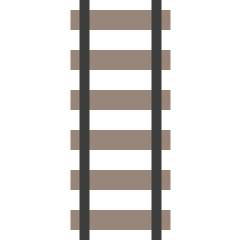
\includegraphics[width=\textwidth]{straight-rail.png}
		\caption{Straight}
		\label{fig:rail-cell-straight}
	\end{subfigure}%
	~
	\begin{subfigure}[t]{.20\linewidth}
		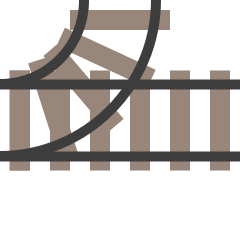
\includegraphics[width=\textwidth]{simple-switch-rail.png}
		\caption{Simple switch}
		\label{fig:rail-cell-simple}
	\end{subfigure}%
	~
	\begin{subfigure}[t]{.20\linewidth}
		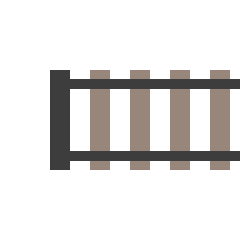
\includegraphics[width=\textwidth]{deadend-rail.png}
		\caption{Deadend}
		\label{fig:rail-cell-deadend}
	\end{subfigure}%
	~
	\begin{subfigure}[t]{.20\linewidth}
		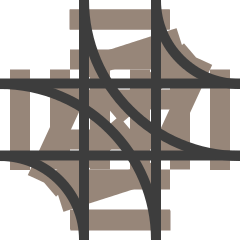
\includegraphics[width=\textwidth]{double-slip-rail.png}
		\caption{Double slip switch}
		\label{fig:rail-cell-double}
	\end{subfigure}%

	\caption{Different \texttt{rail} cell types}
	\label{fig:rail-cells}
\end{figure}

Moreover, \texttt{rail} cells can be occupied by the following entities (the ones shown in figure \ref{fig:agent-target}):
\begin{itemize}
	\item Agent: one \texttt{rail} cell can be seen as a resource with availability equal to one, so that in each time step only one agent can occupy it
	\item Target: each target is statically assigned to one \texttt{rail} cell. Target cells represent the destination of one or more agents (different agents could have the same target). Moreover, the number of possible targets present in the environment is clearly limited by the number of agents
\end{itemize}

\begin{figure}[h]
	\centering
	\captionsetup[subfigure]{justification=centering}
	\begin{subfigure}[t]{.25\linewidth}
		
\includegraphics[width=\textwidth]{agent.png}
		\caption{Agent}
		\label{fig:agent}
	\end{subfigure}%
	~
	\begin{subfigure}[t]{.25\linewidth}
		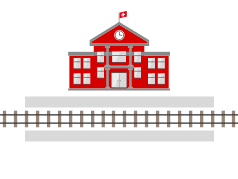
\includegraphics[width=\textwidth]{target.png}
		\caption{Target}
		\label{fig:target}
	\end{subfigure}%
	\caption{Agents and targets}
	\label{fig:agent-target}
\end{figure}

An important fact about the different types of \texttt{rail} cells is that only switches require an agent to make a choice. In Flatland (like in reality) a maximum of two options is available. There does not exist a switch with three or more options.

Finally, every cell that is not \texttt{rail} is \texttt{empty} and neither targets nor agents can fill it up. As shown in figure \ref{fig:env-example}, it is interesting to notice that Flatland is a very sparse environment, meaning that there are a lot more \texttt{empty} cells than \texttt{rail} ones: because of this, representing the environment as a simple dense matrix could lead to overheads and efficiency issues, especially when dealing with relatively big environments.

In the end, the only cell types that we care about are the \texttt{rail} ones: the \texttt{empty} ones are useful only for visualization purposes. Because of this, we could think of representing the environment as a sparse matrix or as a graph containing only \texttt{rail} cells or a subset of them (we will address this issue in section \ref{sec:railway-encoding}).

\begin{figure}[h]
	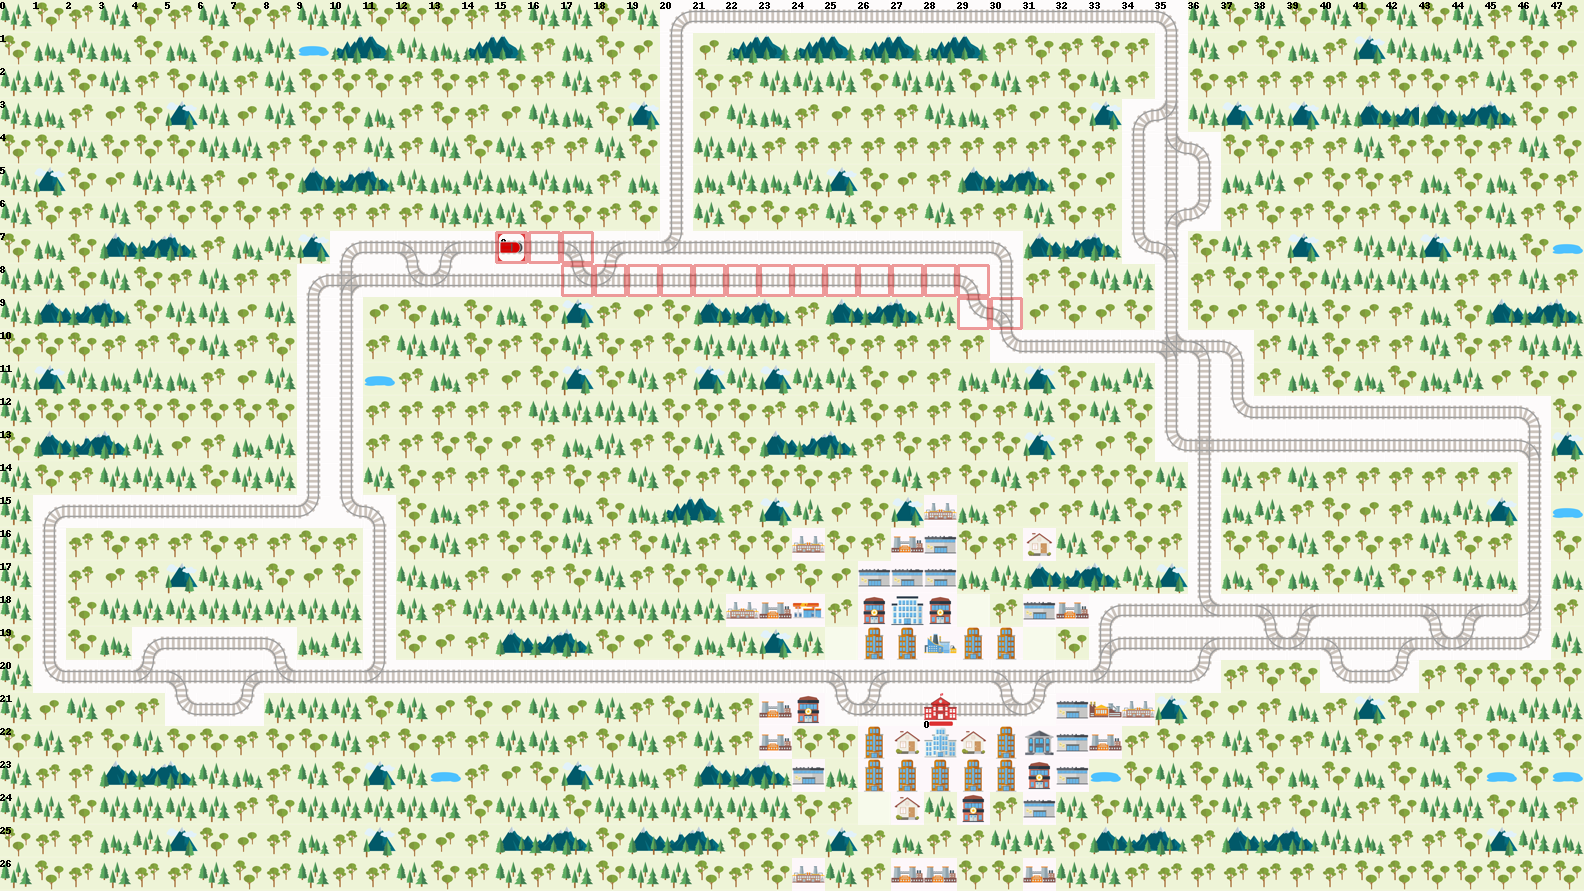
\includegraphics[width=\textwidth]{env.png}
	\caption{An example of a railway environment}
	\label{fig:env-example}
\end{figure}

\subsubsection*{Transitions}
An agent in the Flatland environment is a train that starts from a random \texttt{rail} cell in the map and has to arrive to its assigned target in the minimum number of steps. To do so, the agent can only occupy \texttt{rail} cells.

To move from a cell to another one the agent has to make a choice and, depending on the cell type that they are on and on the connections between cells, an agent can transition from cell $i$, when looking towards direction $d_i$, to cell $j$, looking towards direction $d_j$, if and only if $T_i(d_i, d_j)=1$, where $T_i$ is the transition matrix associated to cell $i$, s.t. $T_i(d_i, d_j)=0$ means that the transition from cell $i$, direction $d_i$ to cell $j$, direction $d_j$ is forbidden (likewise $T_i(d_i, d_j)=1$ means that the transition is allowed). Directions $d_*$ are represented as the $4$ cardinal directions, i.e. North, East, South and West (N, E, S, W), so that each transition matrix $T_*$ can be characterized as a $4\times4$ binary matrix. For example, a deadend cell like the one reported in figure \ref{fig:rail-cell-deadend} would have a transition matrix like the one shown in figure \ref{fig:rail-cell-bitmap}.

\begin{figure}[h]
	\noindent\begin{minipage}{.5\linewidth}
		\begin{equation*}
			\begin{blockarray}{ccccc}
				& N & E & S & W \\
				\begin{block}{c(cccc)}
					N & 0 & 0 & 0 & 0 \\
					E & 0 & 0 & 0 & \mathbf{1} \\
					S & 0 & 0 & 0 & 0 \\
					W & 0 & 0 & 0 & 0 \\
				\end{block}
			\end{blockarray}
		\end{equation*}
	\end{minipage}%
	$\xrightarrow[\text{bitmap}]{\text{to}}$
	\begin{minipage}{.5\linewidth}
		\begin{equation*}
			0000 \; 000\mathbf{1} \; 0000 \; 0000
		\end{equation*}
	\end{minipage}
	\caption{Transition matrix and bitmap of a deadend}
	\label{fig:rail-cell-bitmap}
\end{figure}

As we can observe, only one entry in the matrix has value $1$, meaning that only one transition is possible, i.e. the one s.t. the agent enters heading East and exits heading West.

In the Flatland library, a transition matrix is represented by a bitmap, which can be seen as a linearization by rows of the reported matrix (the mapping between the transition matrix of the deadend cell \ref{fig:rail-cell-deadend} and its bitmap is again shown in figure \ref{fig:rail-cell-bitmap}). In this way, by simply counting the number of true values in the bitmap, we can understand the type of \texttt{rail} cell that we are examining (e.g. only one true value indicates a deadend, while exactly two true values indicate a straight rail).

\subsubsection*{Actions}
Flatland has a discrete action space, meaning that only $5$ possibilities have to be considered at each transition. In particular, Flatland uses the following convention:
\begin{enumerate}
	\item \texttt{MOVE_FORWARD}: the agent maintains the current movement direction, if possible (i.e. if it was heading North, it will continue heading North)
	\item \texttt{MOVE_LEFT}: if the agent is at a switch with a transition to its left, the agent will choose the left path, otherwise the action has no effect (e.g. if the agent was heading North, it will be directed towards East)
	\item \texttt{MOVE_RIGHT}: if the agent is at a switch with a transition to its right, the agent will choose the right path, otherwise the action has no effect (e.g. if the agent was heading North, it will be directed towards West)
	\item \texttt{STOP_MOVING}: the agent remains in the same cell
	\item \texttt{DO_NOTHING}: the agent performs the same action as the last time step
\end{enumerate}

Usually, only a handful of the reported actions can be perfomed on a given cell, meaning that most of the times the actual number of choices is much less than $5$ (we will address this issue in section \ref{sec:real-decisions-choices}).

\subsubsection*{Complications}
The main complications of the Flatland challenge are given by speed profiles, conflicts and malfunctions. In particular, about speed profiles, each and every agent could have a different velocity. The standard speed (and the maximum one) is $1$, which means that the agent crosses one cell in one time step. Speeds can have values in range $(0, 1]$: if an agent has speed $s$, it means that it needs $\lceil\frac{1}{s}\rceil$ time steps to transition from one cell to the next one.

Speeds are assigned to agents based on a custom probability mass function, so that $P(S=s)$ represents the probability that the speed $S$ of an agent is equal to $s$. For example, we could have the following \textit{pmf} (representing a uniform distribution over values $\{\frac{1}{4}, \frac{1}{3}, \frac{1}{2}, 1\}$):

\begin{equation}
	\begin{cases}
		P(S=s) = 0.25 & \text{if } s \in \{\frac{1}{4}, \frac{1}{3}, \frac{1}{2}, 1\} \\
		P(S=s) = 0    & \text{otherwise}
	\end{cases}
\end{equation}

Clearly, the speed factor is a critical one to observe when trying to minimize the total number of time steps in a multi-agent scenario: for example, different agents have to understand that faster ones should go first if a decision has to be made. This is because we would like to avoid bottlenecks of any kind inside the railway network and slower agents can definitely become an issue in an environment with relatively long sequences of straight rails.

About the second complications, i.e. malfunctions, agents can experience defects or failures which do not let them go on in their path towards the target. A malfunction in the Flatland environment is modeled by a Poisson distribution $1 - P_{\lambda}(n=0)=1 - \frac{\lambda^{n}}{n!}\cdot e^{-\lambda}=1 - e^{-\lambda}$, where $\lambda \in (0, 1]$ is the malfunction rate s.t. $\frac{1}{\lambda}$ represents the mean frequency of occurrence of malfunctioning events. For example, if malfunctions are to be expected once every $80$ time steps for an agent, then $\lambda=\frac{1}{80}=0.0125$ and the probability of a malfunction in each time step is equal to $1-e^{-0.0125}=0.01$, while if malfunctions are more rare (e.g. once every $200$ time steps), then we would have a probability value of $1-e^{-0.005}=0.004$. Once an agent is malfunctioning, it stays so for a random number of time steps, bounded by parameters indicating the minimum and maximum duration of a malfunction period.

Again, the malfunction factor is critical, in that it could prevent one or more agents from reaching their targets in the minimum number of time steps. In this way, transitions in the environment become stochastic, thus leading to a slower and much more difficult optimization procedure.

About the third complication, i.e. conflicts, we can define it as a state in which agents cannot perform any action, because they are "blocked" by one or more neighboring agents. Different conflicting situations can arise in practice, where the most basic one is given by two agents heading in different directions in a sequence of straight rails (see figure \ref{fig:two-deadlock}): this situation can in turn cause other deadlocks to happen, as shown in figure \ref{fig:three-deadlock}.

\begin{figure}[h]
	\centering
	\captionsetup[subfigure]{justification=centering}
	\begin{subfigure}[t]{.4\linewidth}
		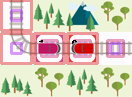
\includegraphics[width=\textwidth]{two-deadlock.png}
		\caption{Two agents}
		\label{fig:two-deadlock}
	\end{subfigure}%
	~
	\begin{subfigure}[t]{.4\linewidth}
		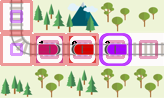
\includegraphics[width=\textwidth]{three-deadlock.png}
		\caption{Three agents}
		\label{fig:three-deadlock}
	\end{subfigure}%

	\caption{Examples of deadlocks}
	\label{fig:deadlocks}
\end{figure}

A full deadlock situation is a state in which every agent is in deadlock: in that case, no agent would be able to arrive at its target. These blocking situations are one of the most intricate and complex factors that should be addressed when designed autonomous agents in the Flatland environment, since they are quite frequent (and they get more frequent as the number of agents increases and the dimension of the grid decreases) and have disastrous consequences (at least in a real-world scenario).

Differently from malfunctions, deadlocks totally prevent agents from reaching their destination: when a malfunction occurs, agents that could previously reach their targets will still be able to reach them once the malfunction period is over, while when a conflict occurs, at least two agents will never arrive at their targets.

\chapter{Environment}
In this chapter we are going to explore better ways to encode the Flatland environment and how agents can interact with these representations.

\section{Railway encoding}\label{sec:railway-encoding}
As already described in chapter \ref{chap:background}, the default Flatland representation was not built with the goal of efficiency in mind, since it stores each and every cell of the 2D grid, while only \texttt{rail} cells are the ones that are actually used by agents. An alternative and more efficient representation could be to use some kind of sparse matrix implementation, where \texttt{empty} cells are not stored at all, but this would only be beneficial from the point of view of memory occupancy, while the usage of more specific data structures could also improve other aspects, like the computation of shortest paths from the agent's position to its target.

In this work, we decided to rely on a graph structure. In particular, we were inspired by the great work described in \cite{jonas} where the author presents the so called Cell Orientation Graph (COG), in which nodes represent cells in the 2D grid as a triple $(x, y, d)$, where $(x, y)$ are the coordinates in the grid (origin in the top-left corner with x-axis looking right and y-axis looking down) and $d$ is one of the four cardinal directions (representing the direction of entrance in the cell). In this way, one \texttt{rail} cell is represented by at most $4$ nodes in the graph: this could seem like a major drawback, but in practice we can observe that the number of nodes is roughly equivalent to the number of cells in the corresponding grid, since we got rid of the \texttt{empty} ones.

Instead, edges in the graph are directed and represent legal transitions, so that no transition matrix or bitmap has to be stored in each node: it is simply encoded in the topology of the network. Moreover, the usage of directed edges greatly simplifies the computation of paths between nodes in the graph.

In order to further simplify the representation of the Flatland environment, we decided to entirely delete nodes which represented straight rails (with the exception of keeping straight rails containing targets and deadends). In this way, what we end up with is something that could be defined a Cell Orientation Junction Graph (COJG), since the remaining nodes are the ones in which an agent either has to make a decision or finishes its trip.

Because of the deletion of almost all nodes associated to straight rails, edges actually represent a connection between an interesting cell and another one (e.g. they link a junction to a target or a junction to a second junction). In order to maintain the same topology as before, the number of deleted straight rails between each pair of interesting nodes is used as the weight of the edge connecting them, so that the computation of shortest paths can automatically take that into account.

Figure \ref{fig:grid-cog-cojg-32x16} shows the comparison, in terms of visual representations, of the standard grid environment and both COG and COJG graphs, in a $32\times 16$ map. In table \ref{table:grid-cog-cojg-32x16} we show the improvements that can be gained by leveraging the usage of the Cell Orientation Graph, and in particular of its modified version, i.e. the Cell Orientation Junction Graph, by computing the number of nodes, edges and \texttt{empty} cells in each representation, in the same $32\times 16$ map of figure \ref{fig:grid-cog-cojg-32x16}.

\begin{figure}[!h]
	\centering
	\captionsetup[subfigure]{justification=centering}
	\begin{subfigure}[b]{.8\linewidth}
		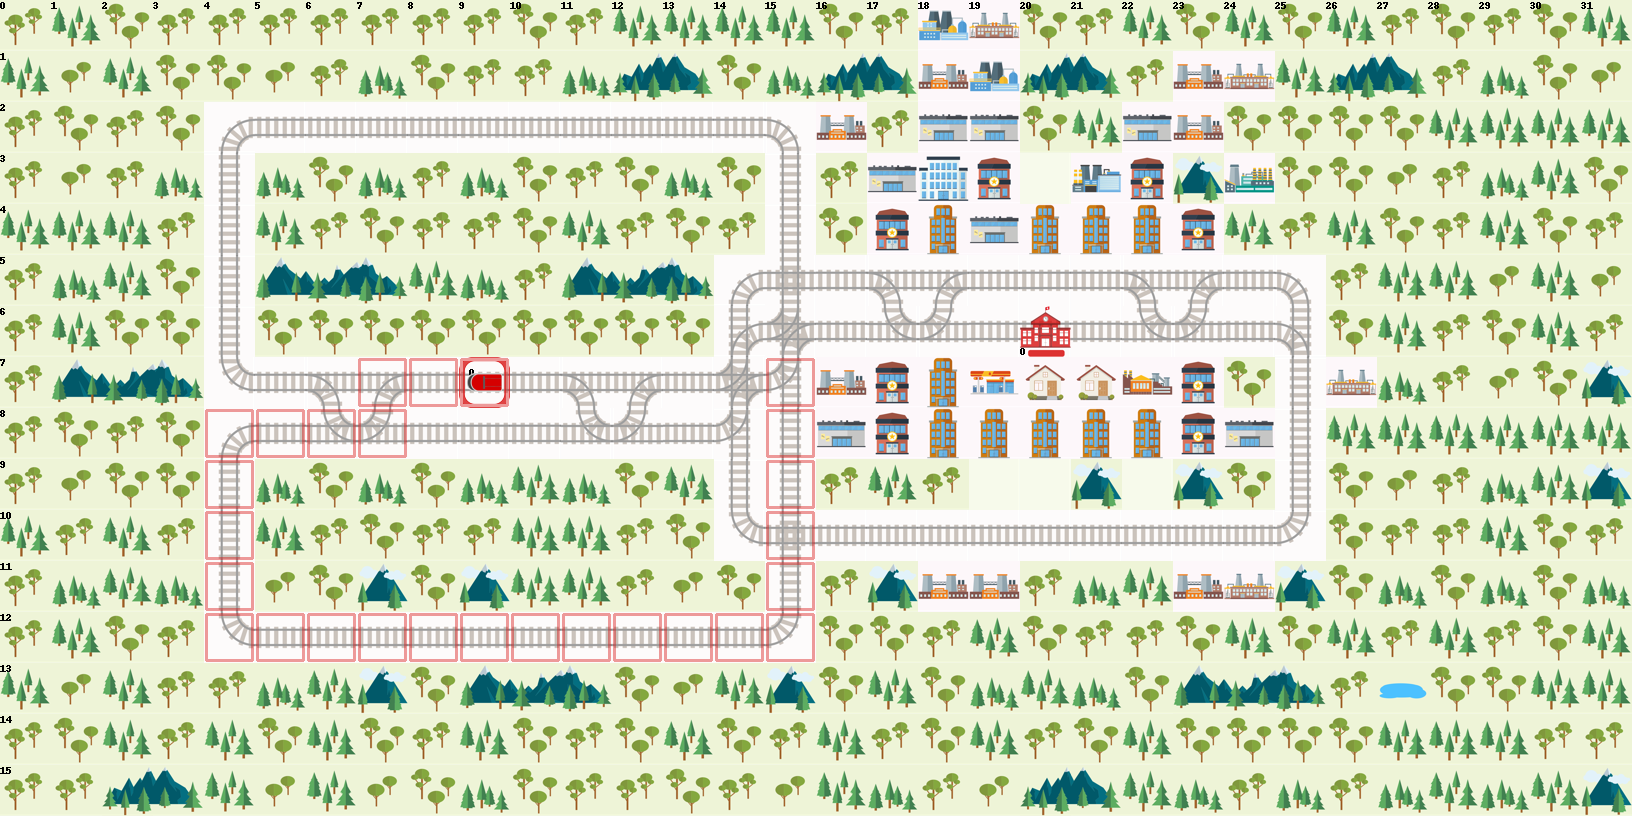
\includegraphics[width=\textwidth]{grid-env-32x16.png}
		\caption{Grid}
		\label{fig:grid-env-32x16}
	\end{subfigure}%

	\begin{subfigure}[b]{.8\linewidth}
		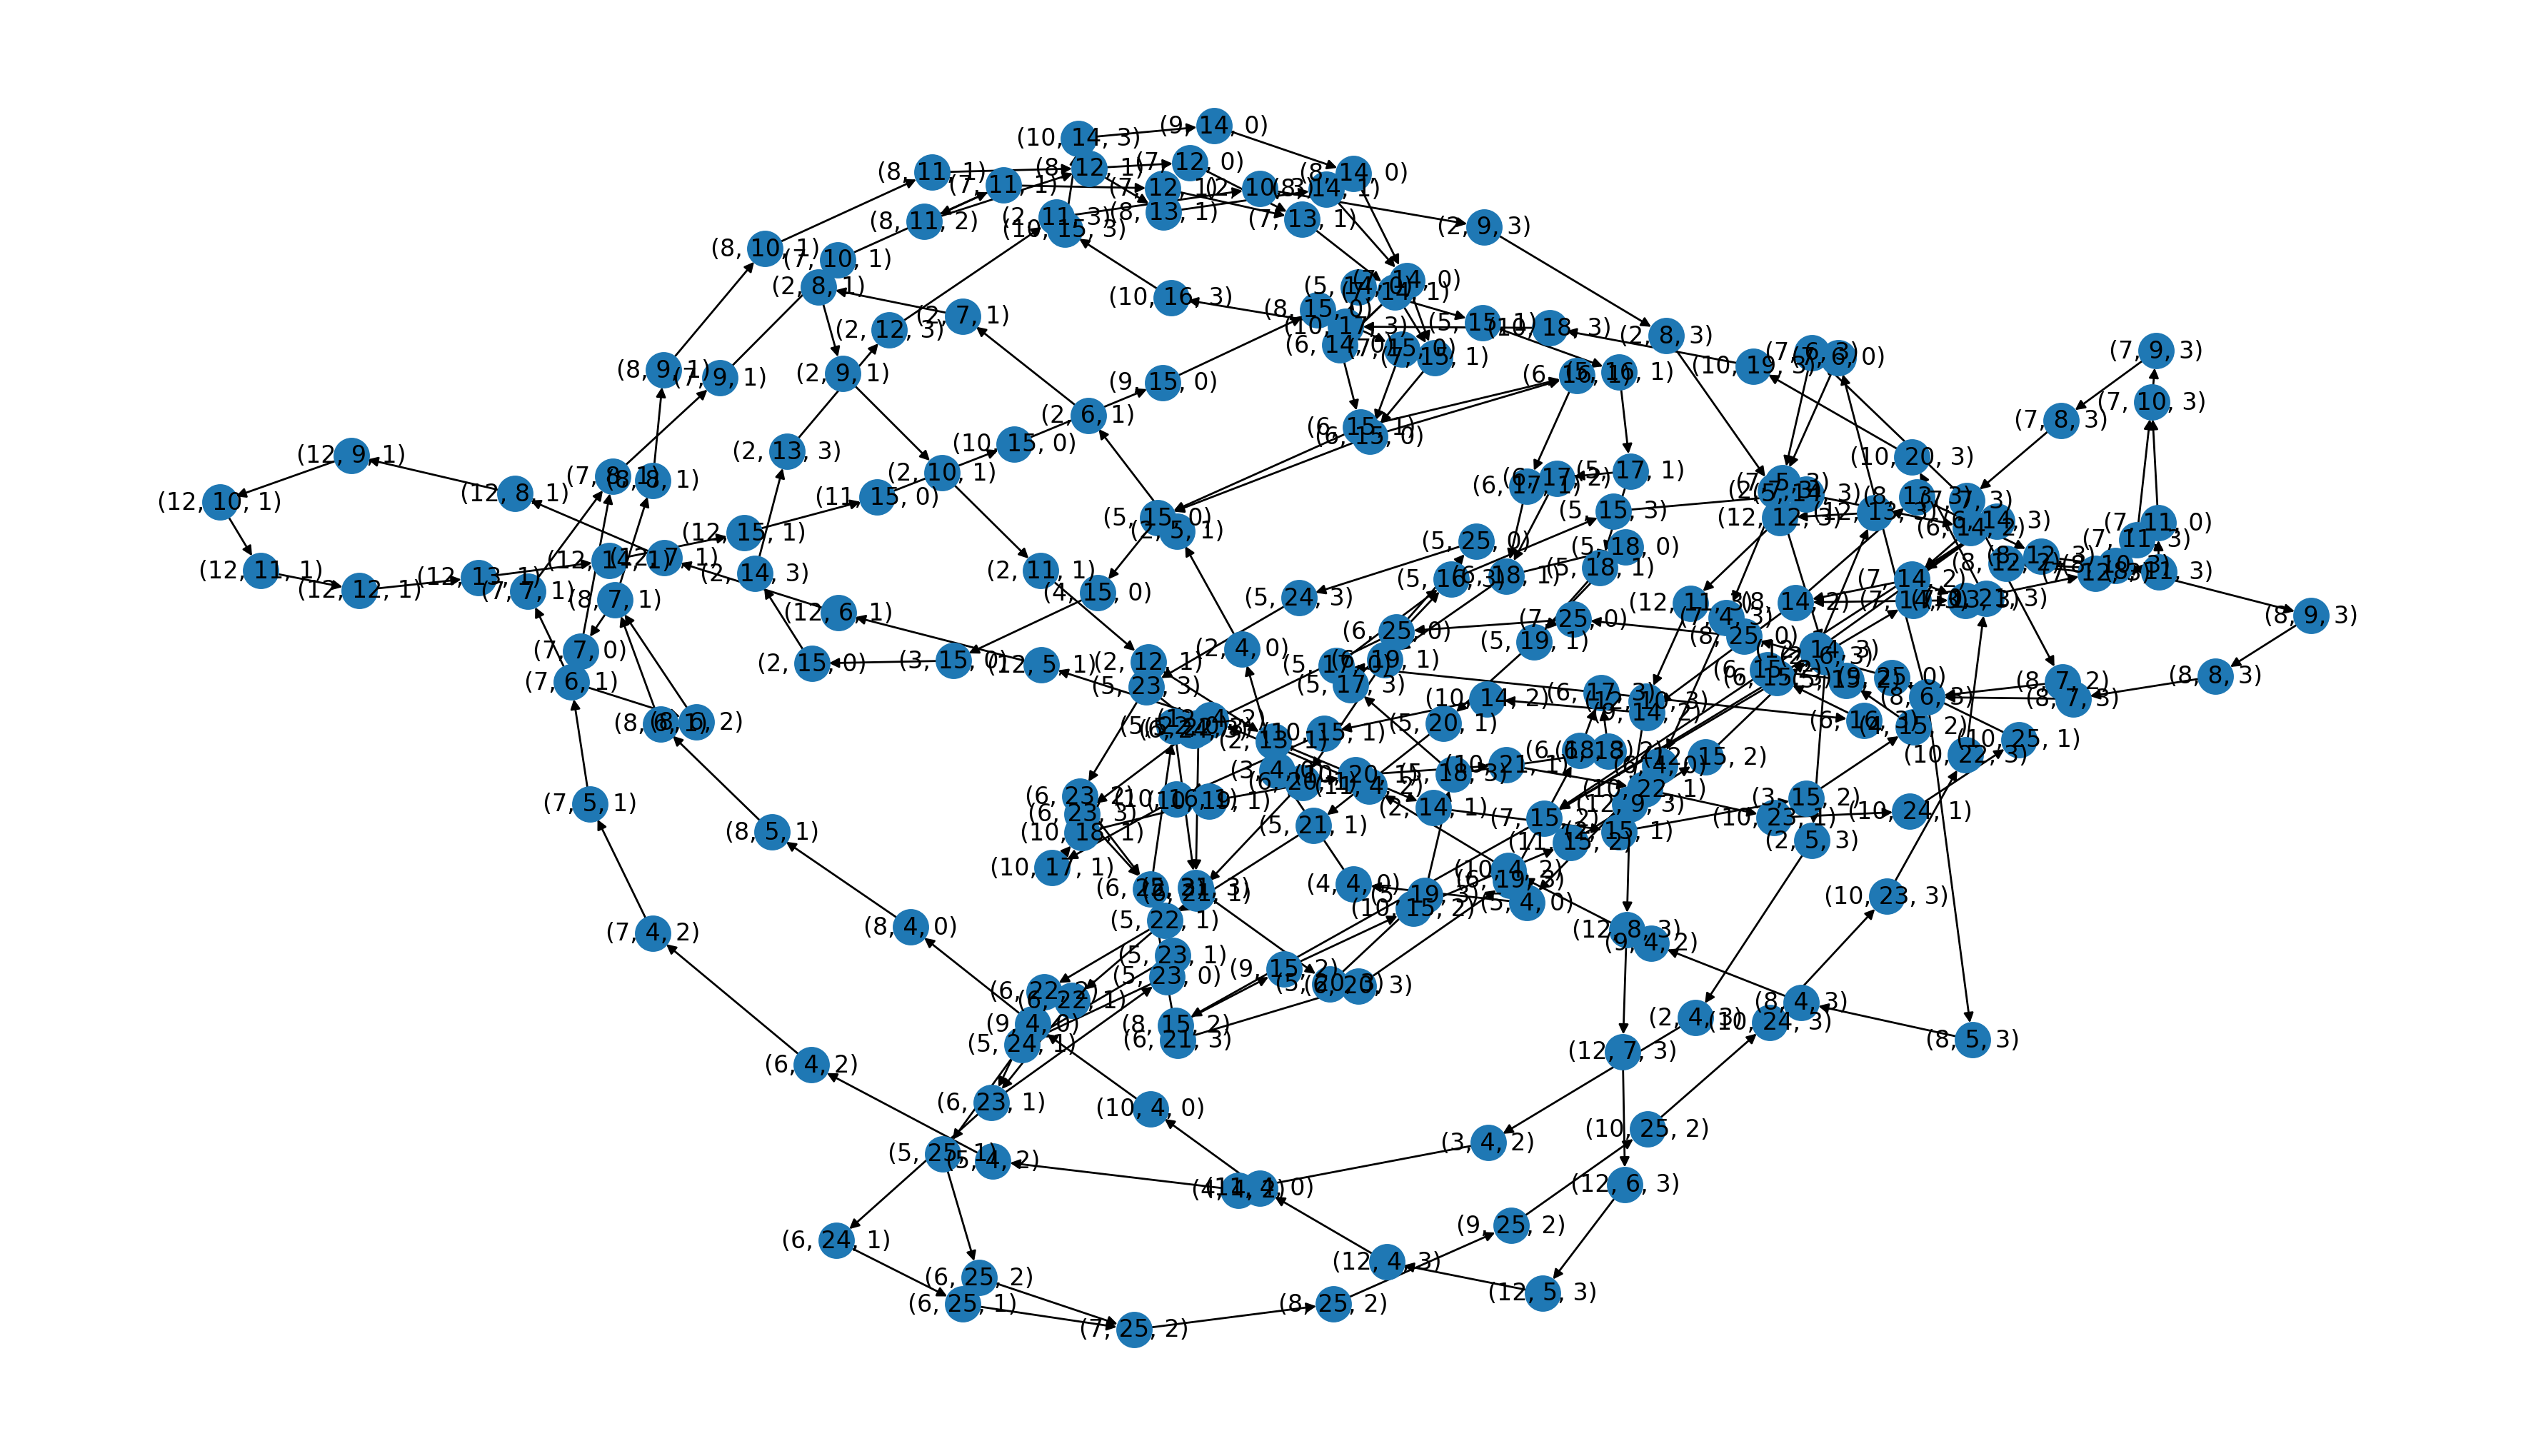
\includegraphics[width=\textwidth]{cog-env-32x16.png}
		\caption{COG}
		\label{fig:cog-env-32x16}
	\end{subfigure}%

	\begin{subfigure}[b]{.8\linewidth}
		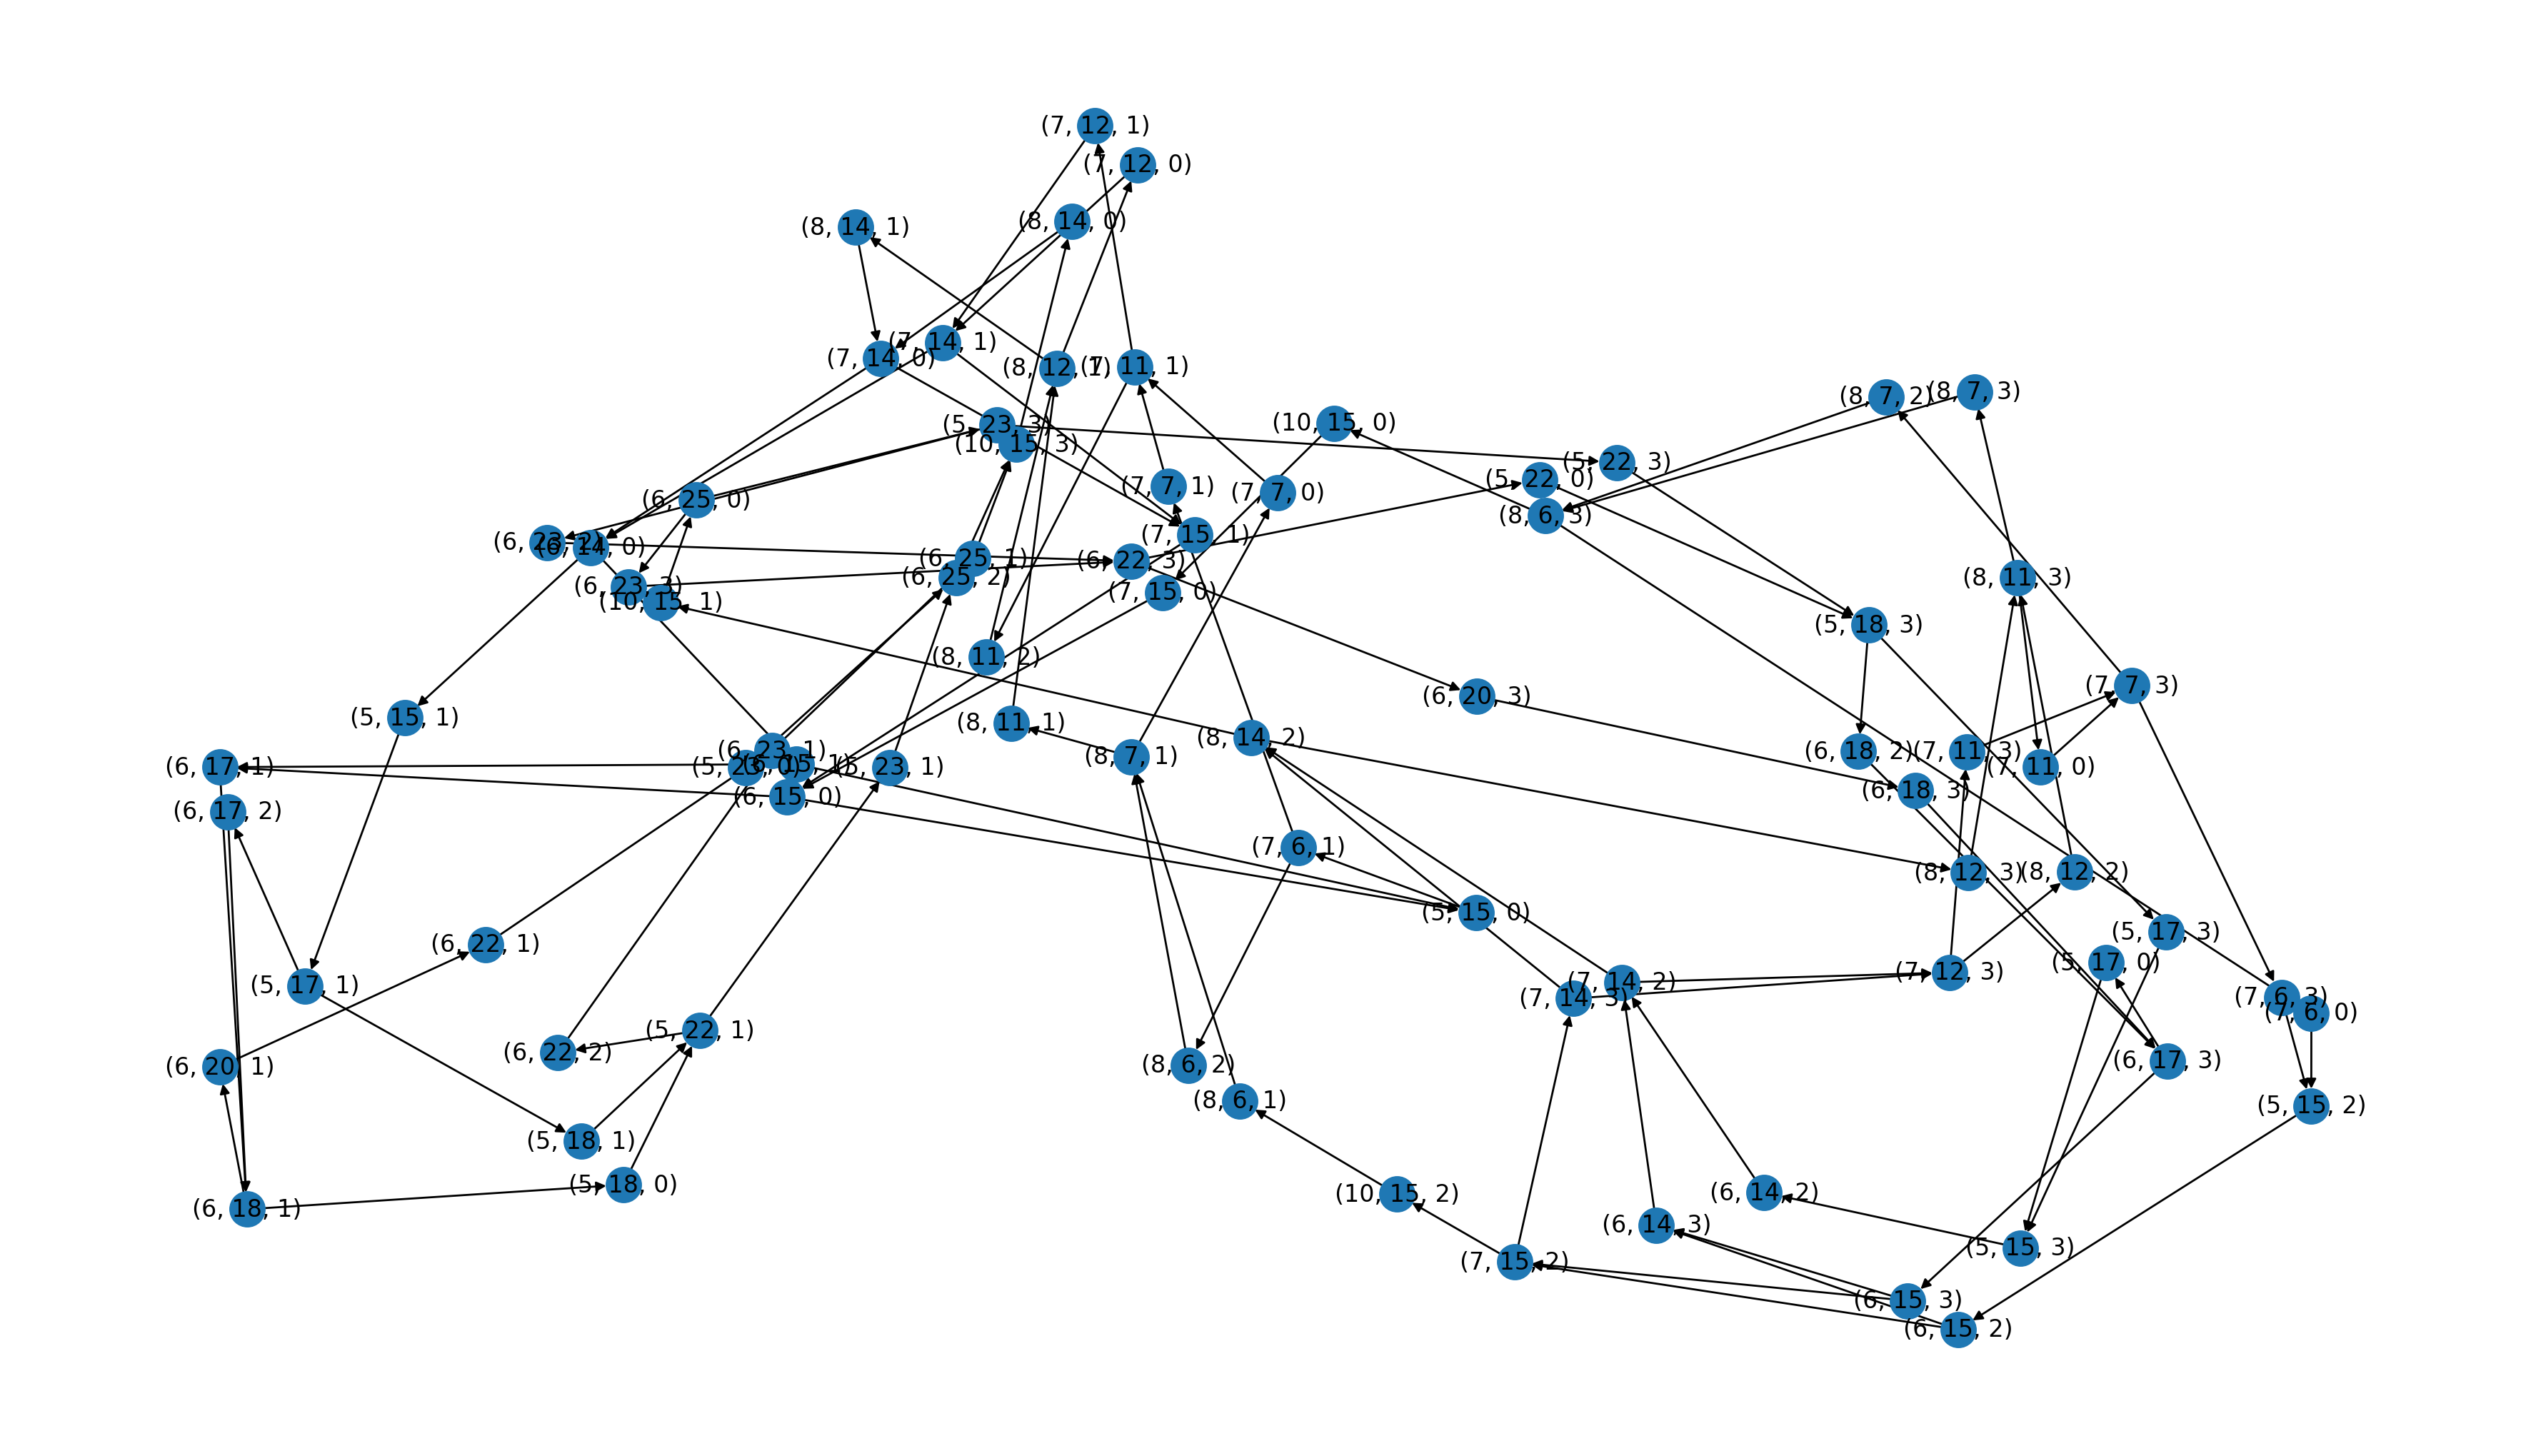
\includegraphics[width=\textwidth]{cojg-env-32x16.png}
		\caption{COJG}
		\label{fig:cojg-env-32x16}
	\end{subfigure}%

	\caption{Different railway encodings of a $32\times 16$ map}
	\label{fig:grid-cog-cojg-32x16}
\end{figure}

\begin{table}[h]
	\center
	\begin{tabular}{||c c c c||}
		\hline
		              & \textbf{Nodes} & \textbf{Edges} & \textbf{Empty} \\ [0.5ex]
		\hline\hline
		\textbf{Grid} & 512            & -              & \num{413}      \\
		\hline
		\textbf{COG}  & 226            & 254            & 0              \\
		\hline
		\textbf{COJG} & 78             & 106            & 0              \\
		\hline
	\end{tabular}
	\caption{Grid, COG, COJG comparison in a $32\times 16$ map}
	\label{table:grid-cog-cojg-32x16}
\end{table}

Since a $32x16$ map is too small to observe big improvements, in figure \ref{fig:grid-cog-cojg-128x64} we also report another example of a sparse grid environment of dimension $128\times64$ and we compare it with its encodings in table \ref{table:grid-cog-cojg-128x64}.

\begin{figure}[!h]
	\begin{subfigure}[b]{\linewidth}
		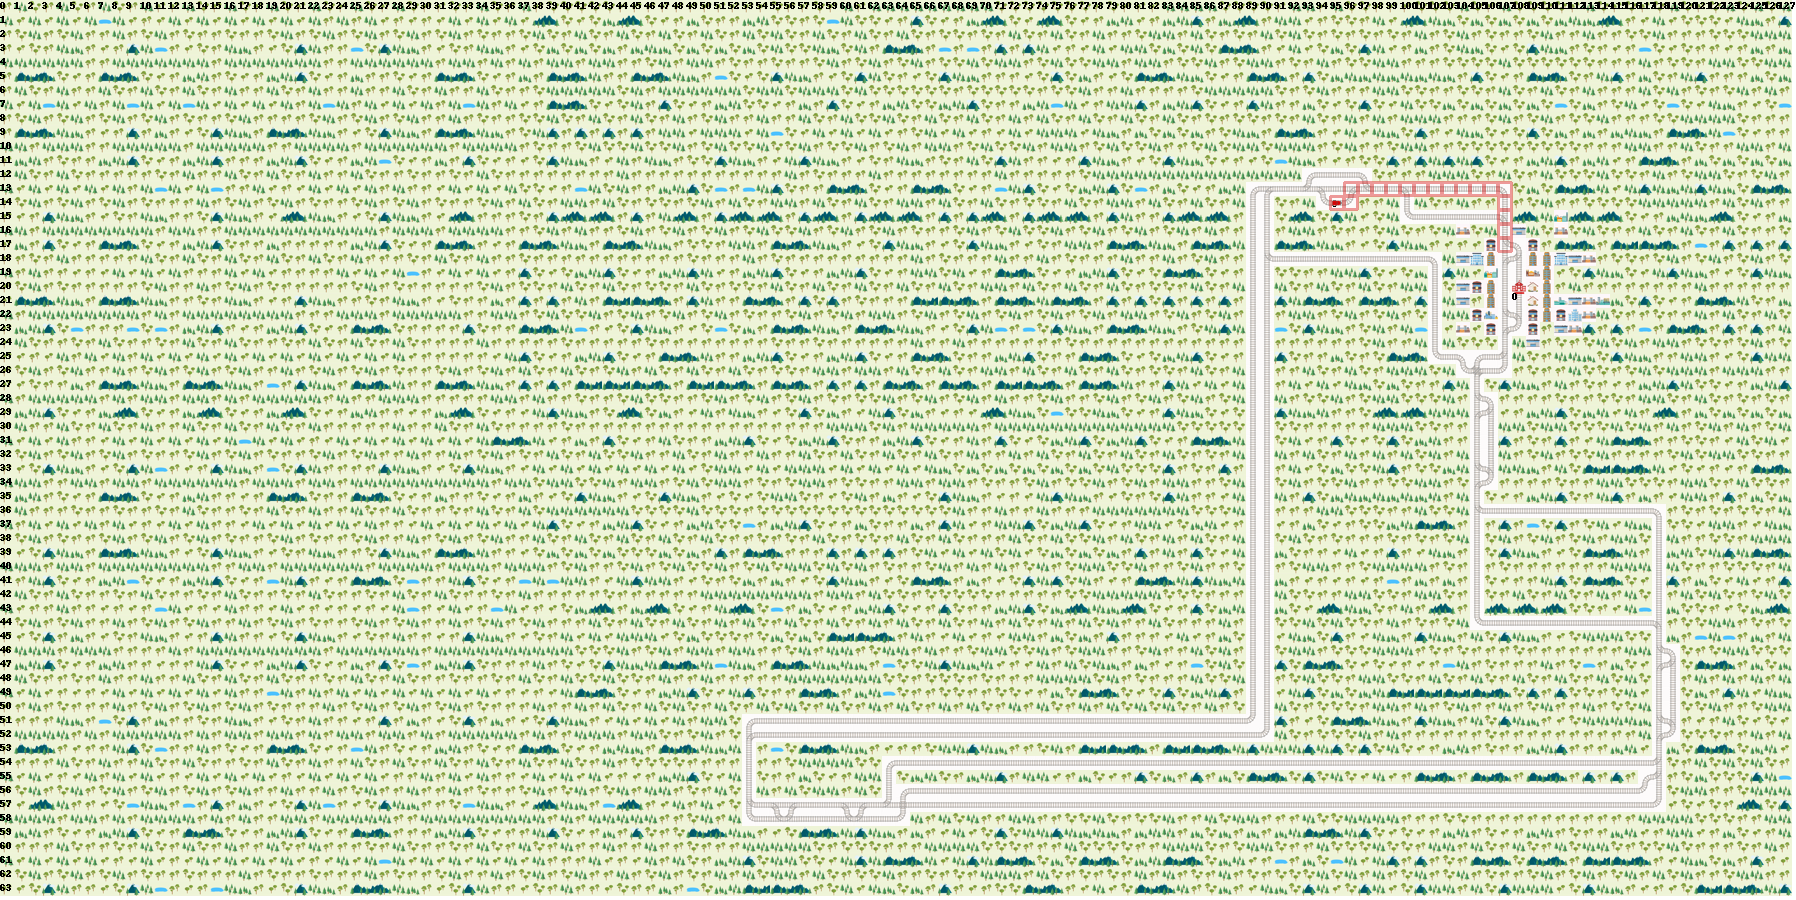
\includegraphics[width=\textwidth]{grid-env-128x64.png}
		\caption{Grid}
		\label{fig:grid-env-128x64}
	\end{subfigure}%

	\begin{subfigure}[b]{\linewidth}
		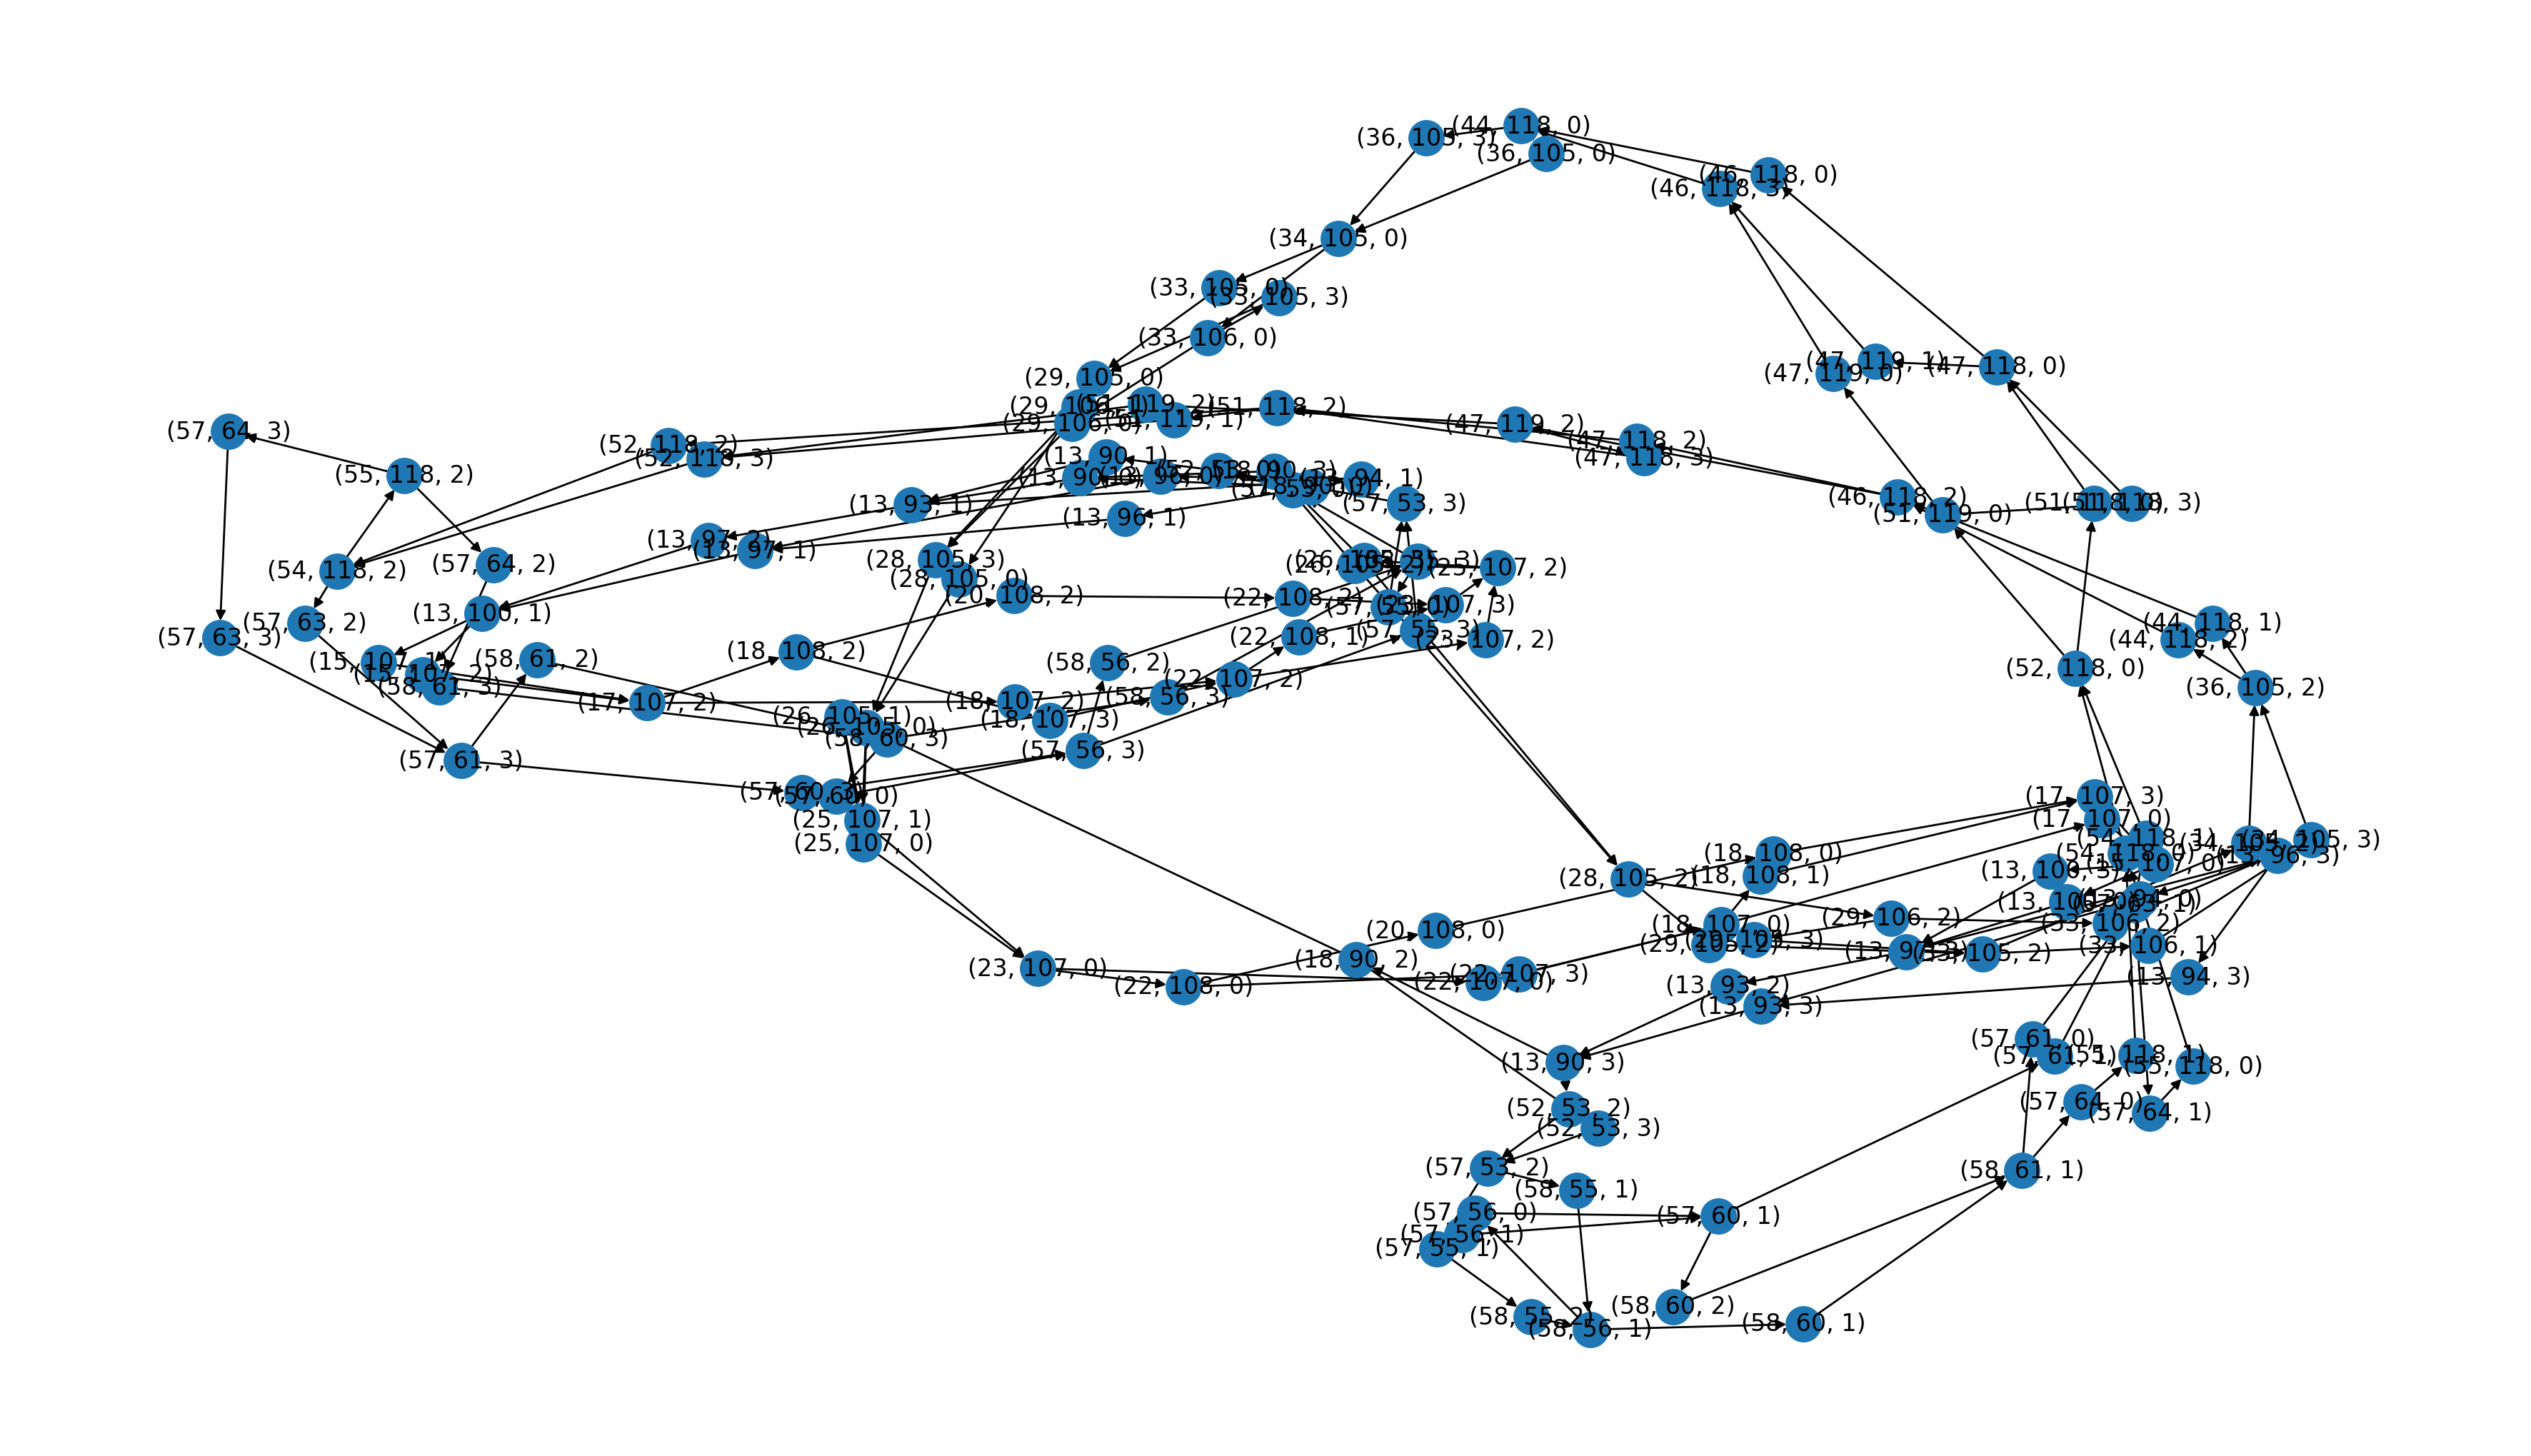
\includegraphics[width=\textwidth]{cojg-env-128x64.png}
		\caption{COJG}
		\label{fig:cojg-env-128x64}
	\end{subfigure}%

	\caption{Grid and COJG comparison in a sparse $128\times64$ map}
	\label{fig:grid-cog-cojg-128x64}
\end{figure}

\begin{table}[h]
	\center
	\begin{tabular}{||c c c c||}
		\hline
		              & \textbf{Nodes} & \textbf{Edges} & \textbf{Empty} \\ [0.5ex]
		\hline\hline
		\textbf{Grid} & \num{8192}     & -              & \num{7732}     \\
		\hline
		\textbf{COG}  & 1050           & 1096           & 0              \\
		\hline
		\textbf{COJG} & 136            & 182            & 0              \\
		\hline
	\end{tabular}
	\caption{Grid, COG, COJG comparison in a $128\times 64$ map}
	\label{table:grid-cog-cojg-128x64}
\end{table}
\clearpage

\section{Predictions}
As reported in Flatland official FAQs, because railway traffic is limited to rails, many decisions that an agent has to take need to consider future situations and detect upcoming conflicts ahead of time. Therefore, Flatland provides the possibility of predictors that predict where agents will be in the future. The stock predictor simply assumes that each agent travels along its shortest path.

\subsection{Shortest and deviation paths}\label{subsec:shortest-deviation-pred}
One of the key advantages of COJG is that it enables us to apply standard shortest path algorithms on directed weighted graphs without any kind of overhead. In particular, we decided to use Dijkstra's algorithm since we do not have negatively weighted edges (in that case, Dijkstra's algorithm could get stuck in a cycle containing at least one edge with negative weight, since it may cycle an infinite number of times and sometimes go down with the total cost as much as it likes).

To build our predictor, we took inspiration from the standard predictor given by the Flatland library as a baseline, which computes shortest paths directly on the 2D grid representation. Our predictor instead takes into account two possibilities: an agent either follows its shortest path or deviates from it. The computation of shortest paths is incremental, meaning that once it is done it only gets updated (i.e. the first node is removed). The only event that causes a re-computation of the shortest path is when the agent makes a choice that does not follow the stored path.

Deviation paths are instead computed on the fly and they represent alternatives from each node of the shortest path. The computation of deviation path $i$, given the shortest path $n_1, \dots, n_i, n_{i+1}, \dots, n_d$, is simply another call to the Dijkstra's routine, where edge $(n_i, n_{i+1})$ is forbidden. In this example, $d$ represents the maximum depth of both shortest and deviation paths.

In this way, the prediction becomes a list of paths, where the first one is the shortest path, composed by at most $d$ nodes, and the following ones are $d-1$ deviation paths, still composed by at most $d$ nodes. When an agent is relatively close to its target (i.e. less than $d$ nodes away from it), the actual path could have a dimension which is less than $d$: to avoid troubles when dealing with dynamically sized vectors, paths are padded to the full depth with special symbols.

In case an agent cannot reach its target anymore, the prediction only comprises a path of two nodes, i.e. the agent's position and the next node in the COJG graph. This mini-path is stored because predictions are used to compute possible deadlocks and, even if an agent cannot arrive at its target anymore, it is still present in the railway environment and it could be a possible source of conflicts.

\section{Real decisions and choices}\label{sec:real-decisions-choices}

\subsection{Real decisions}\label{subsec:real-decisions}
As already hinted in the previous sections, Flatland railway environments are structured in such a way that most of them are composed by long sequences of straight rails, where an agent does not have to commit to any thoughtful choice, but it simply has to follow the path on which it is positioned. The agent is instead required to make a decision in two simple cases: whenever it reaches a fork, i.e. a cell that has more than one successor, or immediately before a join, i.e. before entering another path that crosses its next cell.

Following the reasoning described in \cite{jonas}, we categorize as real decisions those times in which an agent has to select an action when it is positioned in a fork, before a join or in a combination of the two cases. An agent in a fork has to decide on which branch to go next (and ideally, it should not choose to stop on that cell), while an agent before a join has to decide if it wants to stop (maybe to let another agent pass through the join cell) or continue moving.

This idea of introducing real decisions in the Flatland environment greatly reduces the number of calls to the model that is tasked to map states to actions, since the number of real decisions to take is much lower than the number of default actions that one has to provide in the standard framework. In particular, the default number of actions to select is equal to the number of steps that the agent performs in the environment, while the number of real decisions to take is entirely disentagled from the steps parameter, since it is completely dependent on the structure of the environment (e.g. sparser railways tend to have less real decisions w.r.t. denser ones, given the same grid size).

The concept of real decisions leads to a modification in the structure of the COJG graph reported in section \ref{sec:railway-encoding}, so that both types of decisions are encoded as nodes. In particular, COJG is missing most nodes related to cells before a join, since they are usually part of straight rails. Currently, our implementation patches the COJG graph, but a cleaner choice would be to actually add the before join nodes from the start of the building process, which could be something to try for future improvements. 

\subsection{Choices}\label{subsec:choices}
Further analysis related to decisions, again presented in \cite{jonas}, shows a smart action space reduction that could be beneficial to reinforcement learning models. In particular, Flatland uses a discrete action space composed of $5$ actions, which can be reduced to a total of $3$. From now on, we will refer to elements of this new action space as "choices". 

Choices are mapped in such a way that they correspond to the left-most and right-most directions available to the agent at each time-step. In this way, our model only has to predict whether the agent has to follow the track to its left or the track to its right or simply stop. After a choice is selected, it is mapped back to the initial action space by looking at the type of cell the agent is currently on, to ensure compatibility with the Flatland environment.

The new action space is composed by the choices \texttt{CHOICE_LEFT}, \texttt{CHOICE_RIGHT} and \texttt{STOP}.

So, we have to specify two different mappings, the forward and the backward one. The action to choice mapping works as follows:
\begin{enumerate}
	\item If the selected action is \texttt{MOVE_LEFT} and that action is legal from the current cell of the agent, then return \texttt{CHOICE_LEFT}
	\item If the selected action is \texttt{MOVE_RIGHT} and that action is legal from the current cell of the agent, then
	\begin{enumerate}
		\item If only \texttt{MOVE_RIGHT} can be perfomed, then \texttt{CHOICE_LEFT} is returned
		\item Otherwise, \texttt{CHOICE_RIGHT} is returned
	\end{enumerate}
	\item If the selected action is \texttt{MOVE_FORWARD} and that action is legal from the current cell of the agent, then
	\begin{enumerate}
		\item If \texttt{MOVE_LEFT} can be perfomed, then \texttt{CHOICE_RIGHT} is returned
		\item Otherwise, if \texttt{MOVE_RIGHT} can be perfomed, then \texttt{CHOICE_LEFT} is returned
		\item Otherwise, the last resort is \texttt{CHOICE_LEFT}
	\end{enumerate}
	\item If \texttt{STOP_MOVING}, we have a one-to-one mapping with the \texttt{STOP} choice, so that the agent decides to stand still
\end{enumerate}

Instead, the choice to action mapping works as follows:
\begin{enumerate}
	\item If \texttt{CHOICE_LEFT}, then priorities are \texttt{MOVE_LEFT}, \texttt{MOVE_FORWARD}, \texttt{MOVE_RIGHT}
	\item If \texttt{CHOICE_RIGHT}, then priorities are \texttt{MOVE_RIGHT}, \texttt{MOVE_FORWARD}
	\item If \texttt{STOP}, then the only possible outcome is \texttt{STOP_MOVING}
	\item Otherwise, last resort is \texttt{DO_NOTHING}
\end{enumerate}

In the previous bullet points, the word "priority" represents the sequential way in which actions should be selected. For example, if a \texttt{CHOICE_RIGHT} has to be mapped back and \texttt{MOVE_RIGHT} is a legal action from the current cell of the agent, then that action would be selected, otherwise \texttt{MOVE_FORWARD} would be chosen (again, if legal).

\section{Observations}\label{sec:obs}
An observation is a representation of the environment in a particular state. Ideally, this snapshot should be rich enough to convey the right amount of information (so as to distinguish between different configurations), but also small enough that it would be efficient to compute at any given time-step. An observation should also be able to integrate information from local (in our case a train) and global (in our case the grid and all the agents) perspectives.

Flatland provides different observators out of the box (the ones roughly depicted in figure \ref{fig:default-obs}). In particular, the implemented global observation is composed of the following elements:
\begin{itemize}
	\item Transition map tensor with shape $(h, w, 16)$, assuming $16$ bits encoding of transitions
	\item A tensor with shape $(h, w, 2)$, containing the position of the given agent's target in the first channel and the positions of the other agents' targets in the second channel (flag only, no counter)
	\item A tensor of shape $(h, w, 5)$ with the following channels:
	\begin{enumerate}
		\item Agents position and direction
		\item Other agents positions and direction
		\item Agents malfunctions
		\item Agents fractional speeds
		\item Number of other agents ready to depart
	\end{enumerate}
\end{itemize}

The implemented local observation should instead gather information of the rail environment around the given agent. This observation is composed of the following elements:
\begin{itemize}
	\item Transition map tensor of the local environment around the given agent, with shape $(v_h, 2\cdot v_w +1, 16)$, assuming $16$ bits encoding of transitions
	\item A tensor with shape $(v_h, 2\cdot v_w + 1, 2)$ containing the target position of the given agent (if in the agent's vision range) in the first channel and the positions of the other agents' targets (again, if in the agent's vision range) in the second channel
	\item A tensor $(v_h,2\cdot v_w+1, 4)$ containing the one-hot encoding of directions of the other agents at their position coordinates (if in the agent's vision range)
	\item A $4$ elements array with a one-hot encoding of the current direction of the given agent
\end{itemize}
Here, the parameters $v_w$ and $v_h$ define the rectangular view of the agent (of dimension $(2\cdot v_w + 1)\times v_h$) around its position.
One thing to notice about the standard local observation is that it does not contain any clues about the target location, if it's out of range: thus, navigation on maps where the radius of the observation does not guarantee a visible target at all times will become very difficult. 

Moreover, Flatland discourages the use of both the given global and local observations, since the first one does not seem to encode enough information to be effective in a multi-agent scenario, while the second one is simply deprecated in the newest version of their Python library, which makes it practically useless. Because of this, more advanced observations must be used in order to achieve good results on a wide range of environments. In particular, in the following sections we will take a look at another observation present in Flatland library, i.e. the tree observation, and we will use it as the starting point to build our custom binary tree observation, which also integrates all the knowledge and findings that we described in the previous chapters.

\begin{figure}[h]
	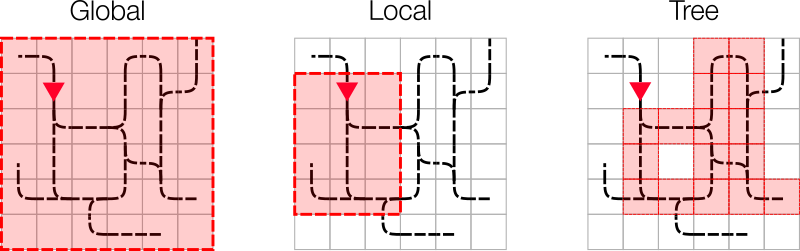
\includegraphics[width=\textwidth]{default-obs.png}
	\caption{Default observators}
	\label{fig:default-obs}
\end{figure}

\subsection{Tree}\label{subsec:tree-obs}
The tree observation is the last one provided out of the box in the Flatland package and it's definitely the most effective overall (w.r.t. the already mentioned global and local ones). This observator builds a tree with arity $4$, s.t. the children of a node always follow a left, forward, right and backward ordering. In particular, a node in the tree represents a deadend, a switch, a target destination or a blank (meaning that no information is carried by that specific node). The children of a node represent its successor nodes when following the left/right/forward branch on a switch or the backward one on a deadend. The mentioned movements are sorted relative to the current orientation of the agent, rather than using standard transition directions (i.e. the four cardinal directions). Whenever a node does not have one of the mentioned successors, that branch becomes useless and gets filled with padding values.

Figure \ref{fig:tree-obs} shows a mapping between a state and the corresponding tree observation, from the point of view of the agent represented by the red triangle. The colors in the figure illustrate what branch the cell belongs to (red means left, pink means forward, green means right and blue means backward). If there are multiple colors in a cell, then this cell will be present multiple times in the tree. The symbols in the figure have instead the following meaning:
\begin{itemize}
	\item Cross: no branch was built, i.e. the parent does not have a valid transition to represent the child
	\item No children: the node is a terminal node (i.e. a deadend, a cell without possible transitions or a leaf of the tree, indicating that the maximum depth was reached)
	\item Circle: a node filled with information
\end{itemize}

\begin{figure}[h]
	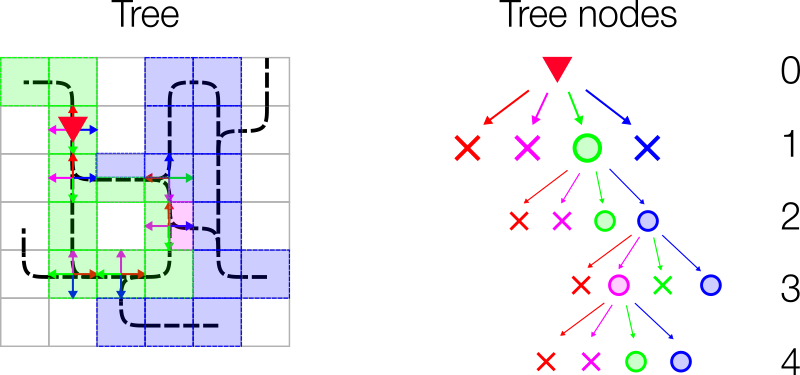
\includegraphics[width=\textwidth]{tree-obs.png}
	\caption{Tree observator}
	\label{fig:tree-obs}
\end{figure}

Whenever a node is valid, it will be packed with the following features:
\begin{enumerate}
	\item If the target of the given agent lies on the explored branch, the current distance from the given agent (in number of cells) is stored
	\item If another agent's target is detected, the distance in number of cells from the given agent's current location is stored
	\item If another agent is detected, the distance in number of cells from the given agent's position is stored
	\item If another agent predicts to pass along this cell at the same time as the given agent, the distance (in number of cells) from the given agent's position is stored
	\item If an unusable switch is detected for the given agent, the current distance (in number of cells) from the given agent's position is stored
	\item Distance in number of cells to the next branching
	\item Minimum distance from the node to the given agent's target, considering the current direction of the agent
	\item Number of agents present in the same direction as the given agent
	\item Number of agents present in the opposite direction as the given agent
	\item Number of time steps that the given agent remains blocked, if a malfunctioning agent is encountered
	\item Slowest observed speed of agents in the same direction as the given agent
	\item Number of agents ready to depart, but not yet active
\end{enumerate}

One key issue related to the described tree observation is related to both time and memory efficiency. In particular, we mentioned a maximum depth parameter that controls how far the observation should reach, in terms of consecutive switches, targets and deadends visited. Clearly, since each node has $4$ children and the output of the observator should be consistent, running it requires to build a complete tree, which we know to have a number of nodes equal to:
$$
n = \sum_{i=0}^{d-1}a^i,
$$
where $d$ is the height of the tree (i.e. our maximum depth) and the arity $a$ is equal to $4$. Just to make a quick example, if $d=7$ then $n=4^0+4^1+4^2+4^3+4^4+4^5+4^6=\num{5461}$. In this way, in the worst case, for each time-step we would have to examine $t\cdot n$ nodes, where $t$ is the number of trains, since one observation is needed for each agent. Following the previous example, in a scenario with $t=10$ agents and a tree observation with depth $d=7$, the reported features should be computed for each of the $\num{5641}\cdot 10=\num{56410}$ analyzed nodes at every time-step. 

\subsection{Binary tree}\label{subsec:binary-tree-obs}
In order to exploit what we've built so far and have an hopefully more efficient computation of each observation, a new observator was created, starting from the same notions described in section \ref{subsec:tree-obs}. 

In particular, our observator builds a feature tensor of shape $(d, d, f)$, where $d$ is the maximum number of hops in the COJG graph to consider and $f$ is the total amount of features for each node. This tensor contains the features of the nodes in the shortest path as the first row and the features of the nodes in the deviation paths (which are exactly $d-1$) as the following rows.

Each node has the following features:
\begin{enumerate}
	\item Number of agents (going in the same direction as the one of the given agent) identified in the subpath from the root up to each node in the path
	\item Number of agents (going in a direction different from the one of the given agent) identified in the subpath from the root up to each node in the path
 	\item Number of malfunctioning agents (going in the same direction as the one of the given agent) identified in the subpath from the root up to each node in the path
	\item Number of malfunctioning agents (going in a direction different from the one of the given agent) identified in the subpath from the root up to each node in the path
	\item Minimum distances from an agent to other agents (going in the same direction as the one of the given agent), in each edge of the path
	\item Minimum distances from an agent to other agents (going in a direction different from the one of the given agent), in each edge of the path
	\item Maximum number of malfunctioning turns of other agents (going in the same direction as the one of the given agent), in each edge of the path
	\item Maximum number of malfunctioning turns of other agents (going in a direction different from the one of the given agent), in each edge of the path
 	\item Distances from the target, from each node in the path
 	\item Path weights (in number of turns) to reach the given node from the root one
 	\item Number of agents using the node to reach their target in the shortest path
 	\item Number of agents in deadlock in the previous path, assuming that all the other agents follow their shortest path
 	\item How many turns before a possible deadlock
 	\item If the node is a fork or not
 	\item How many turns the current agent has been repeatedly selecting the stop action
\end{enumerate}

Initially, we tried to use the feature tensor as our final observation. In particular, we linearized it as a $d\times d \times f$ vector and fed it into one of the neural models that will be described in the next chapters. In this way, the model was not converging to reasonable solutions, since we were ignoring consistency, meaning that in neural models each and every input neuron should always represent the same measure. Instead, since our feature tensor was built by simply considering paths in the environment, one specific node could have represented either the left or the right branch being taken from the previous node, in different runs. This was definitely confusing the agents, so that no convergence was reached.

Because of this, we resorted to the same idea that was presented in \ref{subsec:tree-obs}, but, thanks to the new action space introduced in \ref{subsec:choices}, we were able to shape the feature tensor like a binary tree (i.e. a tree with arity $a=2$), where branches identify choices, i.e. \texttt{CHOICE_LEFT} or \texttt{CHOICE_RIGHT}. One key difference that our custom binary tree has w.r.t. the standard tree observation is the injection of prior knowledge: this is done by filling in values of features that are only related to nodes present either in the shortest or in one of the deviation paths. In this way, the binary tree contains only information about paths that could lead to the agent's target, by completely disregarding the ones that could not. 

Since the resulting tree has half the arity of the one given by Flatland and we still need a complete tree for consistency reasons, let's consider again the example reported in \ref{subsec:tree-obs} to roughly check for efficiency improvements, where a maximum depth of $d=7$ was chosen, with $t=10$ trains. Our complete binary tree would have $n=2^0+2^1+2^2+2^3+2^4+2^5+2^6=\num{127}$ nodes (compared to $\num{5641}$) and the number of total nodes for which features would have to be computed at each time-step would be around $\num{127}\cdot 10=\num{1270}$ (compared to $\num{56410}$). Moreover, the reported number ($\num{1270}$) is an upper bound on the actual number of nodes that should be analyzed, since different time-steps will require different agents to compute an observation, i.e. only those agents that find themselves in a real decision cell.

To sum up efficiency improvements, each feature is built from scratch, by leveraging the performance gains obtained with the COJG graph. Moreover, the observation needs to be computed only when the agent faces a real decision (as described in section \ref{subsec:real-decisions}), since in every other scenario the action that the agent should take is implicit. By combining this with the much lower size of the tree (compared to Flatland's implementation), we are able to compute more observations with less resources overall. Table \ref{table:tree-bt-48x27} shows a comparison of the standard tree observation and our custom binary tree one, in terms of both running times and memory occupancy for a single observation. As we can see, the binary tree observation is around $6$ times faster on average and occupies $30$ times less memory on average than the tree one.

\begin{table}[h]
	\center
	\begin{tabular}{||c c c c c||}
		\hline
					& \multicolumn{2}{c}{\textbf{Time (s)}} & \multicolumn{2}{c||}{\textbf{Memory (MB)}} \\  [0.5ex]
					& \textbf{Avg}         & \textbf{Std}        & \textbf{Avg}          & \textbf{Std} \\  [0.5ex]
		\hline\hline
		\textbf{Tree} & 0.1978 & 0.0199 & 0.4806 & 0.0 \\
		\hline
		\textbf{Binary tree} & 0.0335 & 0.0124 & 0.0153 & 0.0 \\
		\hline       
	\end{tabular}
	\caption{Tree vs. binary tree efficiency in a $48\times 27$ map, with $d=7$}
	\label{table:tree-bt-48x27}
\end{table}

\subsection{Normalization}
We already mentioned that an observation should be considered as a snapshot of a state from the point of view of an agent; then we reported that this snapshot should be consistent across different runs and that it should also be shaped as a tensor of fixed size. All of this pre-preprocessing is a required step that should be carefully considered when working with neural models (the ones that will be described in subsequent chapters). 

Another important aspect about neural networks is that they mostly require input features to be in comparable ranges: this can be achieved by either normalization or standardization. To be clear, the input features that we are talking about are the ones associated to elements of an observation (e.g. a node in our binary tree).

About standardization, a feature $x$ is mapped to $x_s=\frac{x-\mu_x}{\sigma_x}$, where $\mu_x$ and $\sigma_x$ are the mean and standard deviation of feature $x$. In this way, the resulting $x_s$ would have zero mean and standard deviation equal to $1$. One thing to notice, though, is that it requires either to know the underlying distribution of feature $x$ and its corresponding parameters ($\mu_x$ and $\sigma_x$) or a sample of examples from which parameters could be estimated. In the case of reinforcement learning, we definitely do not have pre-computed samples, since we work in an online fashion, meaning that observations are computed on the fly at each time-step and the network gets called with a batch of previously collected observations. Because of this, the only way in which we could standardize features would be to either know the underlying distribution of each one (which is mostly not the case), or use normalization layers in the network itself (e.g. batch normalization \cite{batch-norm} or layer normalization \cite{layer-norm}).

About normalization, it could be used to refer to many different things, but the main idea is again to translate an input range $[l, u]$ to a fixed output range $[min, max]$ (e.g. $[0, 1]$ or $[-1,1]$). Usually, when the input is translated into $[0,1]$ we talk about normalization, while when the input is translated into a range different than $[0,1]$ we talk about min-max scaling. The general formula of min-max scaling is $x_n = l + \frac{x - min}{max - min} \cdot (u - l)$. In the more specific case of default normalization, the formula becomes $x_n = \frac{x}{max}$. 

Normalization enables us to exploit domain knowledge in order to infer ranges for each feature of our observation. In particular, distances are normalized by considering a fixed observation radius as maximum and either zero or the negated radius as minimum (in the case of negative distances, which we used to indicate agents behind the given one, for example), while other features have much clearer ranges (e.g. features related to malfunctions have a minimum at $0$ and a maximum at the maximum duration of a malfunction, which is a parameter of the environment).

\chapter{Reinforcement learning setting}
\subsubsection*{Introduction}
In a single-agent standard reinforcement learning scenario (see figure \ref{fig:rl-single-agent}), the problem is modeled as an MDP (Markov Decision Process), where at each discrete time-step $t$ the agent observes the environment's state $s_t$ (where $s_t \in S$ and $S$ is the whole state space) and takes an action $a_t$ (where $a_t \in A$ and $A$ is the whole action space) that brings it to a new state $s_{t+1}$. Moreover, the agent receives a reward $r_{t+1}$ proportional to the quality of taking action $a_t$ in state $s_t$. Usually, rewards are local, meaning that only the given $(s_t, a_t)$ pair should be considered when computing them. Then, the agent should learn a policy, i.e. a function $\pi: S\times A \rightarrow [0,1]$, that maximizes the expected cumulative return, i.e. $R=\sum_{t=1}^{\infty}\gamma^t r_t$, where $\gamma\in(0,1)$ is the discount rate (a parameter that intuitively encodes how much importance should be given to immediate or future rewards, s.t. $\gamma \rightarrow 0$ favors the former while $\gamma \rightarrow 1$ favors the latter).

\tikzset{
  frame/.style={
    rectangle, draw,
    text width=6em, text centered,
    minimum height=4em,drop shadow,fill=white,
    rounded corners,
  },
  line/.style={
    draw, -{Latex},rounded corners=3mm,
  }
}
\begin{figure}[h]
	\center
	\begin{tikzpicture}[font=\small\sffamily\bfseries,very thick,node distance = 4cm]
		\node [frame] (agent) {agent};
		\node [frame, below=1.2cm of agent] (environment) {environment};
		\draw[line] (agent) -- ++ (3.5,0) |- (environment)
		node[right,pos=0.25,align=left] {action\\ $a_t$};
		\coordinate[left=12mm of environment] (P);
		\draw[thin,dashed] (P|-environment.north) -- (P|-environment.south);
		\pgfmathsetmacro{\Ldist}{4mm}
		\draw[line] ([yshift=-\Ldist]environment.west) -- 
		([yshift=-\Ldist]environment.west -| P) node[midway,above]{$s_{t+1}$};
		\draw[line,thick] ([yshift=\Ldist]environment.west) -- ([yshift=\Ldist]environment.west
		-|P) node[midway,above]{$r_{t+1}$};
		\draw[line] ([yshift=-\Ldist]environment.west -| P) -- ++ (-12mm-\Ldist,0) |- 
		([yshift=\Ldist]agent.west) node[left, pos=0.25, align=right] {state\\ $s_t$};
		\draw[line,thick] ([yshift=\Ldist]environment.west -| P) -- ++ (-12mm+\Ldist,0) 
		|- ([yshift=-\Ldist]agent.west) node[right,pos=0.25,align=left] {reward\\ $r_t$};
	\end{tikzpicture}
	\caption{Single agent RL scenario}
	\label{fig:rl-single-agent}
\end{figure}

Since Flatland is actually a multi-agent environment, the formal definition of the reinforcement learning scenario slightly changes, but the main ideas still hold. As reported in \cite{marl-medium}, MARL (Multi-Agent Reinforcement Learning) typically represents the environment as a stochastic game. While the name is different, it’s fairly similar to an MDP. States become joint states of all the agents, with different rewards corresponding to each possible joint action. Transition functions remain analogous to the single-agent case, replacing states and actions accordingly. 

One of the main challenges of MARL is related to non-stationary transitions, i.e. given a distinct state and action pair, the transition probabilities to other states are not constant (state transitions become dependent on the joint actions of all the agents).

\subsubsection*{Value functions}
As reported in \cite{sutton-barto}, almost all reinforcement learning algorithms involve estimating value functions, i.e. functions of states (or of state-action pairs) that estimate how good it is for the agent to be in a given state (or how good it is to perform a given action in a given state). The notion of “how good” here is defined in terms of future rewards that can be expected, or, to be precise, in terms of expected return. Of course the rewards the agent can expect to receive in the future depend on what actions it will take. Accordingly, value functions are defined with respect to particular ways of acting, called policies (which we already introduced in the previous section).

Formally, the value function of a state $s$ under a policy $\pi$, denoted $V_\pi(s)$, is the expected return when starting in $s$ and following $\pi$ thereafter. For MDPs, we can define $V_\pi$ formally by
$$
V_\pi(s) = \mathbb{E}_\pi\left[G_t\mid s_t=s\right],
$$
where $G_t=\sum_{k=0}^{T}\gamma^{k}r_{t+k+1}$ is the discounted return at time-step $t$ and $E_\pi[\cdot]$ denotes the expected value of a random variable given that the agent follows policy $\pi$.

Moreover, we can also define the value of taking action $a$ in state $s$ under a policy $\pi$, denoted $Q_\pi(s,a)$, as the expected return starting from $s$, taking the action $a$, and thereafter following policy $\pi$:
$$
Q_\pi(s, a) = \mathbb{E}_\pi\left[G_t\mid s_t=s, a_t=a\right],
$$

The relationship between the $V$ and $Q$ functions is as follows:
$$
V_\pi(s)=\sum_a\pi(s,a)\cdot Q_\pi(s,a)
$$

\subsubsection*{Optimal policy}
The main goal of reinforcement learning approaches is to find an optimal policy $\pi^*=\argmax_\pi R$. To do so, different types of algorithms could be employed:
\begin{itemize}
	\item Model-based: the agent tries to understand the world and create a model to represent it, so that, after learning, it could make predictions about what the next state and next reward will be before taking an action
	\item Model-free: they rely on real samples from the environment and never use generated predictions of next state and next reward to alter behaviour
	\begin{itemize}
		\item Value-based: the policy is implicit, so that at each time-step the agent chooses the action that brings it to the next state which has the best evaluation
		\item Policy-based: it avoids forming both the MDP and the value functions, and instead tries to directly learn the (optimal) policy
	\end{itemize}
\end{itemize}

In this work we mainly focused on model-free, value-based techniques. Their goal is to implicitly find the optimal policy, by sequentially pushing the related value functions towards higher quality ones. In this regard, the final aim of our RL agents is to find the optimal action-value function (also called $Q$ function), by leveraging Bellman's optimality equation:
$$
Q^*(s,a)=\max_\pi\mathbb{E}\left[G_t\mid s_t=s,a_t=a,\pi\right]
$$

\section{Rewards and shaping}
Designing rewards is a key property for the success of reinforcement learning agents. Rewards should be simple and straightforward, but they should also encode the right amount of information extracted from the domain of the application. Hence, they cannot be designed in a general fashion, because they are problem-dependent.

Flatland provides the following rewards out of the box:
\begin{itemize}
	\item $-1$ for each step taken
	\item $+1$ when every agent arrives at their target
\end{itemize}

Training agents with the standard reward didn't seem effective in a lot of ways. For example, from our point of view it doesn't make sense to give an agent a reward of $+1$ only if all of them reached their targets. A more sensible idea would be to kind of even out all the negative rewards that the agent got during their journey to the target, but also leaving information about the number of steps that it took to arrive at the destination. 

Backing the reported reasoning, the following rewards shaping was perfomed:
\begin{itemize}
	\item If the agent has arrived to its target, a positive reward equal to the maximum number of steps minus the current number of steps is returned (in this way, if an agent arrives in $n_1$ steps in one execution and in $n_2\le n_1$ steps in another execution, information about the number of steps is not lost and the agent should learn to prefer the transitions that made it receive a reward of $n_2$)
	\item If the agent is in deadlock, a reward equal to the negated maximum number of steps is returned
	\item Because of the introduction of real decisions, rewards have to be accumulated whenever the agent is not in a decision cell (so that, for example, if an agent travels along a sequence of $n$ straight rails, its reward would be equal to $-n$ instead of $-1$ when it exits the sequence)
	\item If an agent performed a stop action, give the agent a reward which is worse than the the reward it could have received by choosing any other action. Then, multiply this weight by the number of turns the agent consequently decided to perform a stop action and compute the product of it with a stop penalty parameter. Finally, this reward is clipped to the maximum value given by a deadlock penalty. In this way, performing a lot of consecutive stop actions has an exponential decrease in the received rewards.
\end{itemize}

\section{Action selection}\label{sec:action-selection}
A reinforcement learning algorithm could be considered as a search algorithm in the huge space of feasible policies. In that case, the aim of our agent would be to travel along the landscape of "policy values" in order to find the global optimum, i.e. the best policy overall. The final goal would thus be to constantly improve the current best policy, via some kind of local search, which in the case of neural networks is implemented using gradient descent.

Because of this local search perspective, another key aspect of the reinforcement learning algorithm is to balance the exploration-exploitation tradeoff. In particular, by exploration we mean probing a large portion of the search space with the hope of finding other promising solutions that are yet to be refined, while exploitation is instead related to the refinement of an already promising solution, by intensifying the search in its neighborhood.

In practical terms, at each time-step an action selector has to decide if the agent should follow the action that our current policy marks as the best one (exploitation) or choose another action (exploration), from the set of available ones.

Moreover, the farther we are in the training process of the RL algorithm the lower should be the exploration parameter, meaning that a decaying mechanism should be implemented to decrease the exploration value at each time-step. Different types of decaying methods could be implemented, like an exponential or a linear one (our experiments were conducted mostly with a linear decay, with a pre-defined number of exploration episodes).

\subsection{$\epsilon$-greedy}
The $\epsilon$-greedy action selector is a standard one in the RL community. It works by treating the $\epsilon$ parameter (which should be in range $[0,1]$) as the probability of exploration, so that $1-\epsilon$ represents the probability of exploitation.

In practical terms, given a random number $r\in[0,1]$ sampled from a uniform distribution and the set of possible actions $A$, the action $a_t$ that is selected at time $t$ is the following:
\[a_t = \left\{
\begin{array}{ll}
      \max_{a\in A} Q_{\pi_t}(s_t,a) & \text{if } r \ge \epsilon \\
      \texttt{random_choice}(A) & \text{if } r < \epsilon \\
\end{array} 
\right., \]
where \texttt{random_choice} is a routine that samples from the given set, with a uniform distribution. 

By tweaking a little bit the $\epsilon$-greedy selector we could also get two other selectors:
\begin{itemize}
	\item Greedy: set $\epsilon=0$ and avoid decaying it (always select the best action)
	\item Random: set $\epsilon=1$ and avoid decaying it (always select a random action)
\end{itemize}

\subsection{Boltzmann}\label{subsec:boltzmann}
The Boltzmann action selector is less common in the RL community. It works by computing a modified softmax of the values associated to actions and using the resulting probability distribution to sample an available action. The balance between exploration and exploitation is controlled by the temperature parameter $\tau$ (which should be in range $(0,1]$), so that higher values of $\tau$ will result in higher exploitation. 

In practical terms, we have to model the probability of each action $a_i$ being selected at time $t$ with the following equation:
$$
P_\tau(a_i) = \frac{exp(Q_{\pi_t}(s_t,a_i) / \tau)}{\sum_{a}exp(Q_{\pi_t}(s_t,a) / \tau)}
$$

Then, a sample is drawn from the set of actions $A$, so that the probability of selecting action $i$ is equal to the previously computed value $P_\tau(a_i)$.

By tweaking a little bit the Boltzmann selector we could also obtain the so-called Categorical action selector, where $\tau=1$ and no decaying is applied to it. In this way, the probability of choosing an action is given by a default softmax over the obtained $Q$ function values.

\section{Action masking}
One important problem that we faced while implementing our agents was related to differenting legal and illegal moves in the learning process. In particular, in the Flatland environment the set of available choices at each time-step is strictly related to the position of the agent: for example, an agent in a straight rail can only decide to follow the path over which it is placed (so only one action would be legal), while an agent that finds itself in a fork would have more than one available actions to choose from.

Computing legal and illegal actions is not a problem in the Flatland environment, since it is fully observable, but injecting this knowledge in the reinforcement learning scheme, so that the agent can learn to avoid illegal moves, is not straightforward. A simple way to do so would be to add a penalty term in the reward, but in this way you are not completely guaranteed that agents will never select an illegal action, because that step would be part of the learning process (i.e. agents would have to learn to avoid those actions).

A more all-round solution would instead completely prevent agents to pick a move that is not available (i.e. agents should directly ignore those actions). To do so, we decided to mask out illegal moves whenever the algorithm has to do some kind of computation or selection on the set of actions. Specifically, in the action selectors we replaced every instance of the $\max$, $\argmax$ and $\softmax$ operator with their ad-hoc masked counterparts and we did the same when computing Bellman optimality.

\chapter{DQN}
A DQN (Deep $Q$-Network), as was first presented in \cite{atari-dqn}, leverages neural networks from the point of view of universal function approximators, to estimate the optimal $Q^*$ state-action function. 

The main idea behind DQN is to estimate $Q^*$ with $Q_\theta$ and use the Bellman equation to update the weights $\theta$ of the network so that $Q_\theta\rightarrow Q^*$. In particular, we will use a regression loss (e.g. MSE or Huber) like the following to minimize the so-called TD (Temporal Difference) error:
$$
L(\theta)=\mathbb{E}_{(s_t,a_t,r_{t+1},s_{t+1})}\left[\left(\underbrace{r_{t+1}+\gamma\max_{a_{t+1}}Q_\theta(s_{t+1}, a_{t+1}) - Q_\theta(s_t, a_t)}_{TD}\right)^2\right]
$$

About the network architecture, the literature does not follow a clear definition, so that the term DQN is mostly linked to the whole training pipeline required to reach good estimates of the optimal $Q$ function. For example, in the original paper \cite{atari-dqn} DeepMind researchers use an initial CNN (Convolutional Neural Network), since their input is represented by videogame frames, followed by an MLP (Multi-Layer Perceptron). In our case, we sticked to just using the final fully-connected layers, as shown in figure \ref{fig:fc-dqn}, where the number of input neurons is given by the linearization of the selected observation, the number of hidden cells and the number of hidden layers are hyperparameters, while the number of outputs is equal to the size of the action space (in our case we have exactly $3$ choices). 

\begin{figure}[h]
	\centering
	\includesvg[width = 200pt]{fc-dqn}
	\caption{Simple DQN example with FC layers}
	\label{fig:fc-dqn}
\end{figure}

Another thing to notice is that the weights used for the target versus the current (presumably non-optimal) $Q$ values are different. In practical terms, a separate network is used to estimate the TD target. This target network has the same architecture as the function approximator but with frozen parameters. Every $T$ steps (a hyperparameter) the parameters from the $Q$-network are copied to the target network. This leads to more stable training because it keeps the target function fixed (for a while). Because of this, assuming $\theta$ to represent the current network weights and $\theta^{-}$ the target network weights, the loss function is updated as follows:
$$
L(\theta)=\mathbb{E}_{(s_t,a_t,r_{t+1},s_{t+1})}\left[\left(r_{t+1}+\gamma\max_{a_{t+1}}Q_{\theta^{-}}(s_{t+1}, a_{t+1}) - Q_{\theta}(s_t, a_t)\right)^2\right]
$$

There are two main ways two copy the weights from the current to the target network:
\begin{enumerate}
	\item Hard update: every $T$ steps, the current network is cloned into the target network
	\item Soft update (or Polyak average): at every time-step a portion of the current weights are shifted onto the target ones, so that at step $i$ we have $\theta_i^{-}=\tau \cdot \theta_i + (1-\tau)\cdot \theta_i^{-}$, where $\tau$ is an hyperparameter that controls the weight transfer amount 
\end{enumerate}

\section{Experience replay}
We already mentioned the problem of non-stationarity related to MARL, when agents have to deal with a stochastic environment, but in practice that same problem is also present in simpler RL algorithms, since the data distribution still changes as the agent learns new behaviours (which is in contrast with the standard assumption of a fixed underlying distribution of deep learning methods). Moreover, we know that supervised learning algorithms assume samples in a dataset to be \textit{i.i.d.} (independent and identically distributed), so that if we model the RL problem as a supervised one (e.g. a DQN can be framed as a regression problem that minimizes the distance from the optimal $Q$ function) we break the independence assumption since sequences of states are usually highly correlated. 

To alleviate the problems of correlated data and non-stationary distributions, in the original DQN formulation \cite{atari-dqn} DeepMind researchers report the use of a data structure named experience replay (also known as replay buffer in the literature), which randomly samples previous transitions, and thereby smooths the training distribution over many past behaviors. In this way, the $(s_t, a_t, r_{t+1}, s_{t+1})$ tuple shown in the previous loss equations should be considered as a sample extracted from the current replay buffer.

In practical terms, there are two main ways to implement an experience replay $E$:
\begin{itemize}
	\item Uniform \cite{atari-dqn}: previous experiences are drawn from a uniform distribution $\sim U(E)$
	\item Prioritized \cite{per}: authors propose to more frequently replay transitions with high expected learning progress, as measured by the magnitude of their TD error
\end{itemize}

\section{Improvements}
\subsection{Double}\label{subsec:double-dqn}
One important issue of standard DQNs is that they tend to overestimate $Q$ values (which is mostly due to the $\max$ operator in the Bellman optimality equation), leading to unstable training and low quality policies. 

In order to mitigate the issue, in \cite{double-dqn} they propose to decouple the selection of an action from its evaluation. From a practical point of view, we only have to change how the TD error is computed:
$$
L(\theta)=\mathbb{E}_{(s_t,a_t,r_{t+1},s_{t+1})}\left[\left(r_{t+1}+\gamma Q_{\theta^-}(s_{t+1},\argmax_{a \in A}Q_\theta(s_{t+1},a)) - Q_{\theta}(s_t, a_t)\right)^2\right]
$$

Intuitively, in double DQNs we are mitigating the overestimation bias by adding a second estimator, so that chances of both estimators being overoptimistic at the same action are simply lower. In this way, estimator $Q_{\theta}$ would "obtain the best action", while $Q_{\theta^-}$ would evaluate the $Q$ values for the estimated action, so as to average out the inherent noise.

\subsection{Dueling}\label{subsec:dueling-dqn}
The main goal of dueling architectures, as first presented in \cite{dueling-dqn}, is still to solve the overestimation problem described in \ref{subsec:double-dqn}. Moreover, since for most applications it seems unnecessary to know the value of each action at every timestep, the dueling architecture can learn which states are valuable and which are not, without having to learn the effect of each action for each state.

In particular, authors rely on the fact that the $Q$ function can be decomposed in the sum of two functions, the value function $V$ and the advantage function $A$, so that $Q_\pi(s,a)=V_\pi(s)+A_\pi(s,a)$. Moreover, from the expression of the state-value function $V_\pi(s)=\mathbb{E}\left[Q_\pi\left(s,a\right)\right]$ it follows that $\mathbb{E}\left[A_\pi\left(s,a\right)\right]=0$.

From a practical point of view, a dueling DQN can be implemented by separating the $Q$ function estimation into two streams, the "value" and "advantage" one (as shown in the last layers in figure \ref{fig:dueling-dqn}), to then recombine them into a single output which represents the $Q$ estimates themselves.

The recombination layer cannot simply be the sum of the presumed "value" and "advantage" outputs, since they actually aren't reliable estimates of the mentioned functions and they suffer from lack of identifiability (meaning that, given a $Q$ value we are not able to recover the corresponding $V$ and $A$ values uniquely), as thoroughly described in \cite{dueling-dqn}. To this end, authors decided to force the advantage function estimator to have zero advantage at the
chosen action, so that output merging could be computed by the following formula:
$$
Q(s,a)=V(s) + \left(A(s,a) - \max_{a'\in A}A(s,a')\right)
$$

An alternative formulation of the recombination layer is to use the average (instead of the maximum) over the advantage function. In this way, the original semantics of $V$ and $A$ are lost, but authors report that it eases optimization, while still preserving the relative rank of the $A$ (and hence the $Q$) values. Formally:
$$
Q(s,a)=V(s) + \left(A(s,a) - \frac{1}{|A|}\sum_{a'\in A}A(s,a')\right)
$$

\begin{figure}[h]
	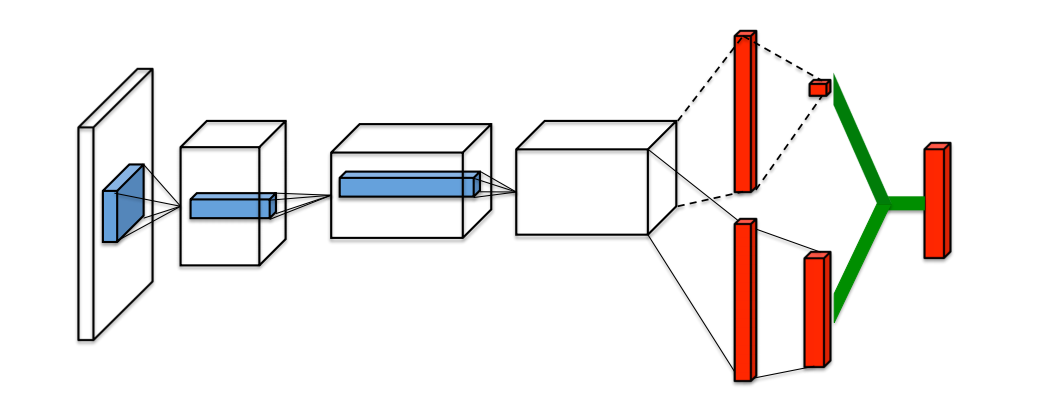
\includegraphics[width=\textwidth]{dueling-dqn.png}
	\caption{Dueling DQN architecture}
	\label{fig:dueling-dqn}
\end{figure}

\subsection{Gradient noise reduction}
\citeauthor{atari-dqn} observed that large gradients can be detrimental to the optimization of DQNs. This was noted in the context of large reward values, but it is possible that overestimation bias can also introduce variance in the gradient and have a negative effect overall.

To solve this issue, in \cite{atari-dqn} authors decided to clip gradient values to a fairly small range (fixed to be $[-1,1]$), while in \cite{per} they went for a solution which clips the norm of the gradient to a specific maximum value (which was chosen to be $10$).

By further inspecting the rationale behind \citeauthor{atari-dqn} (quoted below), we can conclude that using an MSE loss and clipping gradient values to be in $[-1,1]$ should give the same results as using an Huber loss without any kind of gradient noise reduction. However, it's not clear if \citeauthor{per} followed the same reasoning.
\begin{displayquote}
	We also found it helpful to clip the error term from the update to be between $-1$ and $1$. Because the absolute value loss function $|x|$ has a derivative of $-1$ for all negative values of $x$ and a derivative of $1$ for all positive values of $x$, clipping the squared error to be between $-1$ and $1$ corresponds to using an absolute value loss function for errors outside of the $(-1,1)$ interval. This form of error clipping further improved the stability of the algorithm.
\end{displayquote}

\subsection{Bellman operators}
So far, we sticked to training the presented models with the reported losses, by having Bellman optimality in mind. As already discussed in \ref{subsec:double-dqn} and \ref{subsec:dueling-dqn}, the main goal of the authors that developed the double and dueling DQN improvements was to reduce the overestimation bias of the resulting $Q$ values, which is mainly due to the use of the $\max$ operator in Bellman's equation.

In \cite{softmax-bellman}, \citeauthor{softmax-bellman} explore the possibility of directly modifying Bellman's equation to understand if a change in the $\max$ operator therein could be beneficial to the $Q$ function estimates and how this could impact their overoptimistic behavior.

In particular, other Bellman operators had already been presented, but the main two on which authors decided to focus are $\softmax$ and $\mellowmax$. The latter was first conceived in \cite{mellowmax-bellman} to be used as either an alternative action selector (see section \ref{sec:action-selection}) or directly inside Bellman equation. Formally, the $\mellowmax$ operator can be written as
$$
mm_\omega(s) = \frac{1}{\omega}log\left(\frac{1}{|A|} \sum_{a'\in A} exp(\omega \cdot Q(s,a'))\right),
$$ 
where $\omega$ is a tuning parameter. \citeauthor{mellowmax-bellman} show that $\mellowmax$ converges to $\mean$ and $\max$ when $\omega\rightarrow 0$ and $\omega\rightarrow \infty$, respectively. Moreover, they also prove that $\mellowmax$ is a contraction, which means that the same convergence properties guaranteed for the $\max$ operator in Bellman's equation still hold. The main disadvantage of $\mellowmax$ is that it doesn't directly provide a probability distribution over actions, so that additional steps are needed to properly inject it into Bellman optimality.

About the other operator discussed in \cite{softmax-bellman}, it leverages a $\softmax$ modified to account for an additional temperature $\tau$ parameter (as already shown in \ref{subsec:boltzmann}), so that when $\tau\rightarrow 0$ we get back the standard Bellman equation. In practical terms, the softmax Bellman operator can be implemented by modifying how the TD error is computed, by substituting the $\max$ computation with the following formula:
$$
\sum_{a_{t+1}}\frac{exp(Q_{\theta^-}(s_{t+1}, a_{t+1})/\tau)}{\sum_{\hat{a}}exp(Q_{\theta^-}(s_{t+1}, \hat{a})/\tau)}\cdot Q_{\theta^-}(s_{t+1},a_{t+1})
$$

Even though $\softmax$ Bellman is not a contraction (as shown in \cite{softmax-contraction} with a counterexample), experiments reveal that its usage can improve test scores over standard double and dueling DQNs with certain temperature values. Moreover, authors in \cite{softmax-bellman} generally observed higher maximum scores and faster
learning than their $\max$ counterparts: this already suggests that the $\softmax$ operator can mitigate the overestimation bias.

However, depending upon the amount of noise, it is possible that, unlike double DQN, the reduction caused by $\softmax$ could exceed the bias introduced by $\max$ (overcompensation). But, when combined with double Q-learning, this effect becomes very small.

In our experiments, the use of the $\softmax$ Bellman operator 

\chapter{GNN}
The main idea behing GNNs (Graph Neural Networks) is, given an input graph, to map its nodes into an embedding space and use the embedded vectors to perform some kind of downstream task (e.g. node classification or link prediction). 

GNN architectures take inspiration from CNNs (Convolutional Neural Networks), by focusing on a local portion of the input data, thus recycling the idea of shared weights. Actually, GNNs are usually framed as a general framework that pops up more and more often in different specialized deep learning architectures: for example, the original transformer \cite{transformers} designed for NLP tasks operates on fully connected graphs representing all connections between the words in a sequence (see \cite{gnn-transformers} for a generalization of transformers which leverages the graph connectivity inductive bias).

Formally, given an input graph $G=(V,E)$, where $V$ is the vertex set, $E$ is the edges set ($E\subseteq V\times V$), we denote with $A$ the adjacency matrix of $G$, so that $a_{i,j}=w\neq 0$ if and only if node $i$ is connected to node $j$ via the edge $(i, j)$ that weighs $w$ (otherwise $a_{i,j}=0$). Moreover, we define feature matrices $X_V\in \mathbb{R}^{|V|\cdot n}$ and $X_E\in \mathbb{R}^{|E|\cdot m}$, where $n$ is the number of features associated to each node and $m$ is the number of features associated to each edge.

\section{Integrating GNNs in DQNs}
In the literature, there have been lots of promising work towards the integration of GNNs and DQNs, where experiments show great generalization results over graph-structured input data.

In \cite{dqn-gnn-routing} authors study the problem of finding the optimal routing configuration for a set of traffic demands (which is NP-hard). Their solution relies on a centralized approach, where the agent has a global view of the current state and is tasked to route messages in an end-to-end fashion. In this scenario, the routing problem is defined as finding the optimal routing policy for each incoming source-destination traffic demand and the learning process is guided by an objective function that aims to maximize the traffic volume allocated in the network in the long-term. The GNN part comes into play with the state representation itself, where the graph is directly defined by the underlying network and features are attached to links between nodes (e.g. the current available capacity).

In \cite{dgn} and \cite{dqn-gnn-robot} authors rely on a different perspective of the input graph, which, instead of being an encoding of the input data, it's used as a form of local communication between agents. In particular, in their decentralized setting each node in the graph is an agent and the links to other agents are determined by a distance metric, so that the actual neighborhood of a node changes over time. Features are instead computed by specialized architectures (sequences of CNNs and MLPs), starting from raw local observations. In this way, both the topology of the network and the features associated to each node evolve together with the multi-agent environment, so that the overall model should be able to adapt to this dynamicity. 

\section{Architectures}
\subsection{Entire graph embeddings}
Recalling the railway encoding described in \ref{sec:railway-encoding}, where the environment is represented as a compact graph, the observations described in \ref{sec:obs} do not seem effective enough at exploiting all the underlying knowledge already encoded in the topology of the network. Up to now, the shortest/deviation paths predictor (see \ref{subsec:shortest-deviation-pred}) and the binary tree observator (see \ref{subsec:binary-tree-obs}) relied on the COJG graph only as a way to gain running time efficiency. Because of this, different experiments were made to try and extract features from the COJG graph itself.

\subsection{Multi-agent graph embeddings}

\chapter{Results}

\chapter{Conclusions}

\printbibliography

\end{document}
